
% This LaTeX was auto-generated from MATLAB code.
% To make changes, update the MATLAB code and republish this document.

\documentclass{article}
\usepackage{graphicx}
\usepackage{color}

\sloppy
\definecolor{lightgray}{gray}{0.5}
\setlength{\parindent}{0pt}

\begin{document}

    
    
\section*{Examples of how to specify `MeshBoundaryCoordinates' to generate various types of FE meshes}

\begin{par}
Note that when using �a, the call to genmesh2d is not needed as this call is done from within �a But you can define the `MeshBoundaryCoordinates' in exactly the same way within the input file `Ua2D\_InitiaUserInput.m'
\end{par} \vspace{1em}
\begin{par}
To run individual examples you can use the matlab option of running code sections from within editor. See: 'doc run code sections' Just click on some part of the code using the mouse, the text will be highligted in yellow, then press ctrl ret
\end{par} \vspace{1em}

\subsection*{Contents}

\begin{itemize}
\setlength{\itemsep}{-1ex}
   \item example: simple polygon
   \item example: periodic boundary conditions
   \item example: sinusoidal bed
   \item example\% ice dome
   \item example:  house withouth a window
   \item example: a house with a window! :-)
   \item a house with a tree
   \item a house with windows and a tree
   \item mesh with several holes and islands
\end{itemize}


\subsection*{example: simple polygon}

\begin{par}
mesh boundary coordinates should go clockwise around the domain (although if this is done incorrectly, �a will automatically correct for this anyhow.)
\end{par} \vspace{1em}
\begin{verbatim}
CtrlVar=Ua2D_DefaultParameters(); %

% Note; When creating this mesh using �a, only the following
% three lines are required in the Ua2D_InitialUserInput.m
CtrlVar.MeshSizeMax=0.1;
CtrlVar.MeshSizeMin=0.1;
MeshBoundaryCoordinates=[-1 -1 ; -1 0 ; 0 1 ; 1 0 ; 1 -1 ; 0 0];

[MUA,FEmeshTriRep]=genmesh2d(CtrlVar,MeshBoundaryCoordinates);
figure ;  PlotFEmesh(MUA.coordinates,MUA.connectivity)
drawnow
%str=input('Next example? y/n [y] ? ','s');  if strcmpi(str,'n') ; return ; end
\end{verbatim}

        \color{lightgray} \begin{verbatim} Creating an input file for gmesh : GmeshFile.geo 
Calling gmesh with GmeshFile.geo as a geo input file, and creating GmeshFile.msh output file 
The gmesh call is:  C:\cygwin64\home\Hilmar\ghg\Ua\gmsh-2.11.0-Windows\gmsh.exe GmeshFile.geo -2 -v 1  
Loading GmeshFile.msh 
 Reading GmeshFile.msh.  
Mesh Type : 2.2 0 8 Reading nodes done.  Reading elements done.
 No inside-out elements. 
  \end{verbatim} \color{black}
    
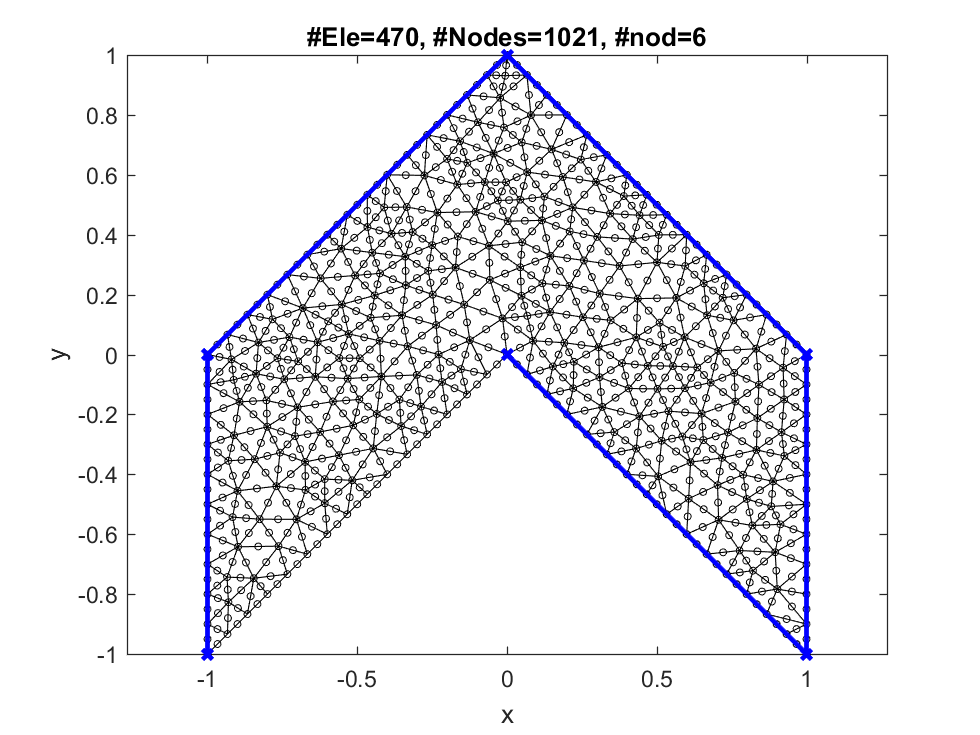
\includegraphics [width=4in]{ExamplesOfMeshGeneration_01.eps}


\subsection*{example: periodic boundary conditions}

\begin{verbatim}
CtrlVar=Ua2D_DefaultParameters();
L=20e3 ; H=1e3;
CtrlVar.MeshSizeMax=H/10;
CtrlVar.MeshSizeMin=CtrlVar.MeshSizeMax/10;
MeshBoundaryCoordinates=[0 0 ; 0 H ; L H ; L 0];
% these lines are added to the gmsh .geo input file each time such a file is created
CtrlVar.GmshGeoFileAdditionalInputLines{1}='Physical Line(1) = {1};';
CtrlVar.GmshGeoFileAdditionalInputLines{2}='Physical Line(2) = {2};';
CtrlVar.GmshGeoFileAdditionalInputLines{3}='Physical Line(3) = {3};';
CtrlVar.GmshGeoFileAdditionalInputLines{4}='Physical Line(4) = {4};';
CtrlVar.GmshGeoFileAdditionalInputLines{5}='Physical Surface(1) = {1};';
CtrlVar.GmshGeoFileAdditionalInputLines{6}='Periodic Line {1,2} = {3,4};';
% now everything needed for mesh generation has been defined

[MUA,FEmeshTriRep]=genmesh2d(CtrlVar,MeshBoundaryCoordinates);
figure ;  PlotFEmesh(MUA.coordinates,MUA.connectivity)
drawnow

%str=input('Next example? y/n [y] ? ','s');  if strcmpi(str,'n') ; return ; end
\end{verbatim}

        \color{lightgray} \begin{verbatim} Creating an input file for gmesh : GmeshFile.geo 
Calling gmesh with GmeshFile.geo as a geo input file, and creating GmeshFile.msh output file 
The gmesh call is:  C:\cygwin64\home\Hilmar\ghg\Ua\gmsh-2.11.0-Windows\gmsh.exe GmeshFile.geo -2 -v 1  
Loading GmeshFile.msh 
 Reading GmeshFile.msh.  
Mesh Type : 2.2 0 8 Reading nodes done.  Reading elements done.
 No inside-out elements. 
  \end{verbatim} \color{black}
    
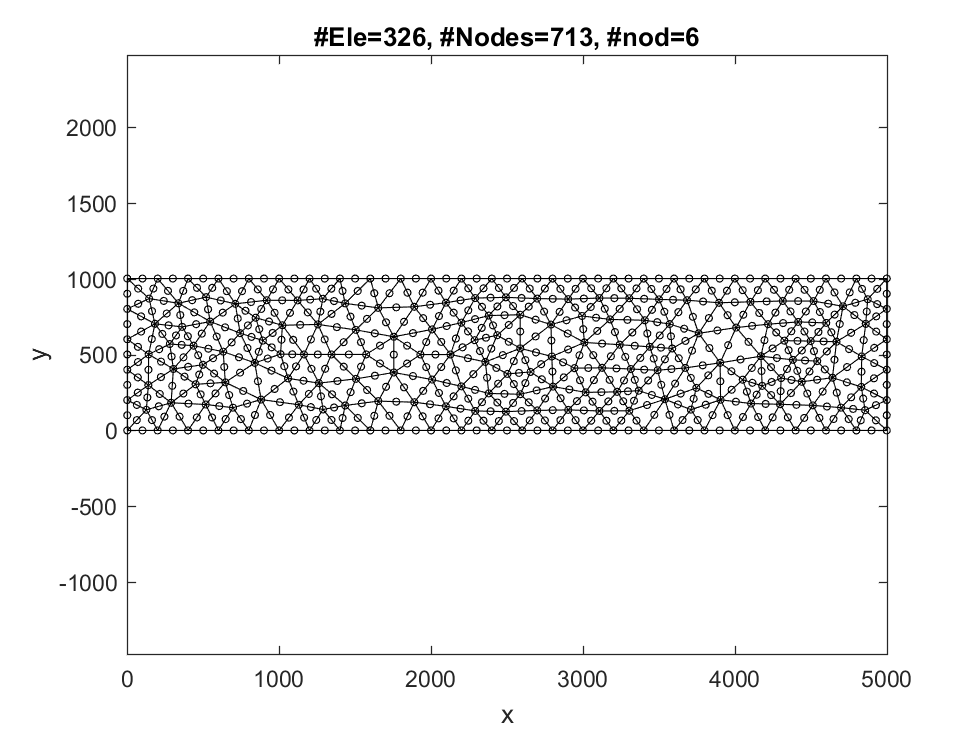
\includegraphics [width=4in]{ExamplesOfMeshGeneration_02.eps}


\subsection*{example: sinusoidal bed}

\begin{verbatim}
CtrlVar=Ua2D_DefaultParameters();
xL=-20e3 ; xR=20e3 ; yB=0 ; yT=2e3;
lambda=(xR-xL)/2; Ampl=1e3 ;
CtrlVar.MeshSize=0.5e3;
CtrlVar.MeshSizeMin=CtrlVar.MeshSize/5;
CtrlVar.MeshSizeMax=5*CtrlVar.MeshSize;
CtrlVar.GmeshCharacteristicLengthExtendFromBoundary=1;
CtrlVar.GmeshCharacteristicLengthFromCurvature = 1 ;

xbed=xL:CtrlVar.MeshSize:xR;
ybed=Ampl*sin(2*pi*xbed/lambda)+  yB;
xbed=xbed(:) ; ybed=ybed(:);

MeshBoundaryCoordinates=[xR yB ; xR yT ; xL yT ; xL yB ; xbed(2:end-1) ybed(2:end-1) ];
N=length(xbed)+2;
% these lines are added to the gmsh .geo input file each time such a file is created
CtrlVar.GmshGeoFileAdditionalInputLines{1}='Periodic Line {1} = {3};';
CtrlVar.GmshGeoFileAdditionalInputLines{2}='Physical Line(0) = {1};';
CtrlVar.GmshGeoFileAdditionalInputLines{3}='Physical Line(1) = {2};';
CtrlVar.GmshGeoFileAdditionalInputLines{4}='Physical Line(2) = {3};';
CtrlVar.GmshGeoFileAdditionalInputLines{5}=['Physical Line(3) = {4:',num2str(N),'};'];
CtrlVar.GmshGeoFileAdditionalInputLines{6}='Physical Surface(1) = {1};';

[MUA,FEmeshTriRep]=genmesh2d(CtrlVar,MeshBoundaryCoordinates);
figure ;  PlotFEmesh(MUA.coordinates,MUA.connectivity)
drawnow

%str=input('Next example? y/n [y] ? ','s'); if strcmpi(str,'n') ; return ; end
\end{verbatim}

        \color{lightgray} \begin{verbatim} Creating an input file for gmesh : GmeshFile.geo 
Calling gmesh with GmeshFile.geo as a geo input file, and creating GmeshFile.msh output file 
The gmesh call is:  C:\cygwin64\home\Hilmar\ghg\Ua\gmsh-2.11.0-Windows\gmsh.exe GmeshFile.geo -2 -v 1  
Loading GmeshFile.msh 
 Reading GmeshFile.msh.  
Mesh Type : 2.2 0 8 Reading nodes done.  Reading elements done.
Warning: Negative determinant in all elements
   
 All elements are inside out. All elements therefore flipped. 
   No longer all elements inside out. 
   No inside-out elements. 
  \end{verbatim} \color{black}
    
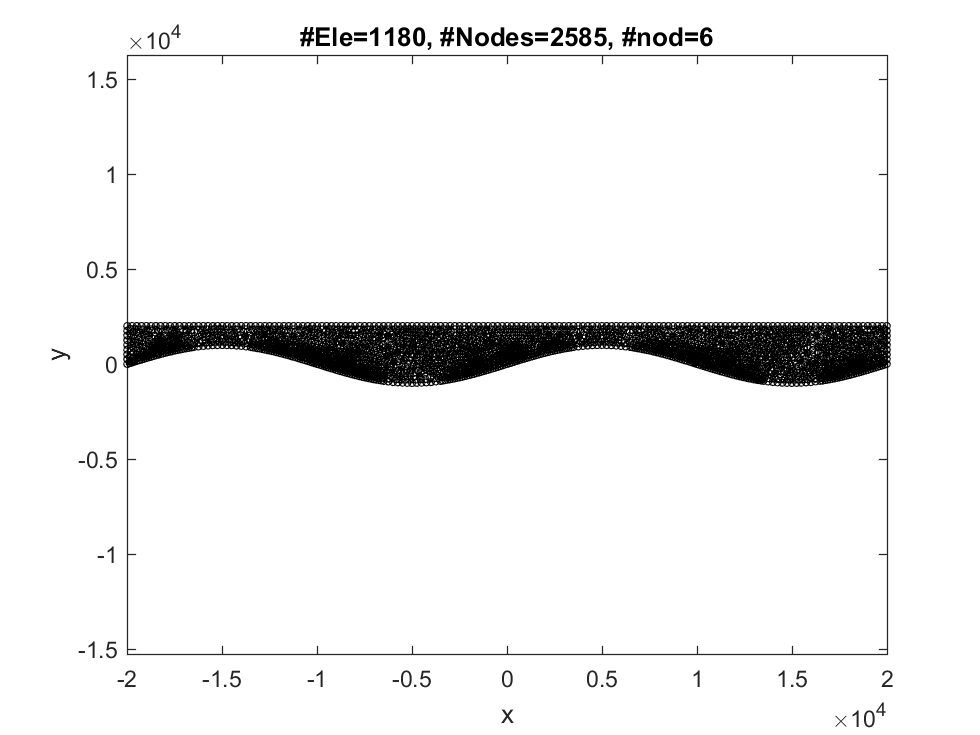
\includegraphics [width=4in]{ExamplesOfMeshGeneration_03.eps}


\subsection*{example\% ice dome}

\begin{verbatim}
CtrlVar=Ua2D_DefaultParameters();
L=20e3; h0=250;
xL=-L ; xR=L ; yB=0 ;  s0=3e3;

gamm=-s0/L^2;
CtrlVar.MeshSize=1e3;
CtrlVar.MeshSizeMin=0.1e3;
CtrlVar.MeshSizeMax=1e3;

xSurf=xL:CtrlVar.MeshSize:xR;
ySurf=s0+gamm*(abs(xSurf)).^2;
N=numel(xSurf);

%MeshBoundaryCoordinates=[L 0 ; -L 0 ; xSurf(:) ySurf(:)+100];
MeshBoundaryCoordinates=[xSurf(:) ySurf(:)];
% these lines are added to the gmsh .geo input file each time such a file is created
CtrlVar.GmshGeoFileAdditionalInputLines{1}=['Physical Line(1) = {',num2str(N),'};'];
CtrlVar.GmshGeoFileAdditionalInputLines{2}='Physical Surface(1) = {1};';

[MUA,FEmeshTriRep]=genmesh2d(CtrlVar,MeshBoundaryCoordinates);
figure ;  PlotFEmesh(MUA.coordinates,MUA.connectivity)
drawnow
%str=input('Next example? y/n [y] ? ','s'); if strcmpi(str,'n') ; return ; end
\end{verbatim}

        \color{lightgray} \begin{verbatim} Creating an input file for gmesh : GmeshFile.geo 
Calling gmesh with GmeshFile.geo as a geo input file, and creating GmeshFile.msh output file 
The gmesh call is:  C:\cygwin64\home\Hilmar\ghg\Ua\gmsh-2.11.0-Windows\gmsh.exe GmeshFile.geo -2 -v 1  
Loading GmeshFile.msh 
 Reading GmeshFile.msh.  
Mesh Type : 2.2 0 8 Reading nodes done.  Reading elements done.
 No inside-out elements. 
  \end{verbatim} \color{black}
    
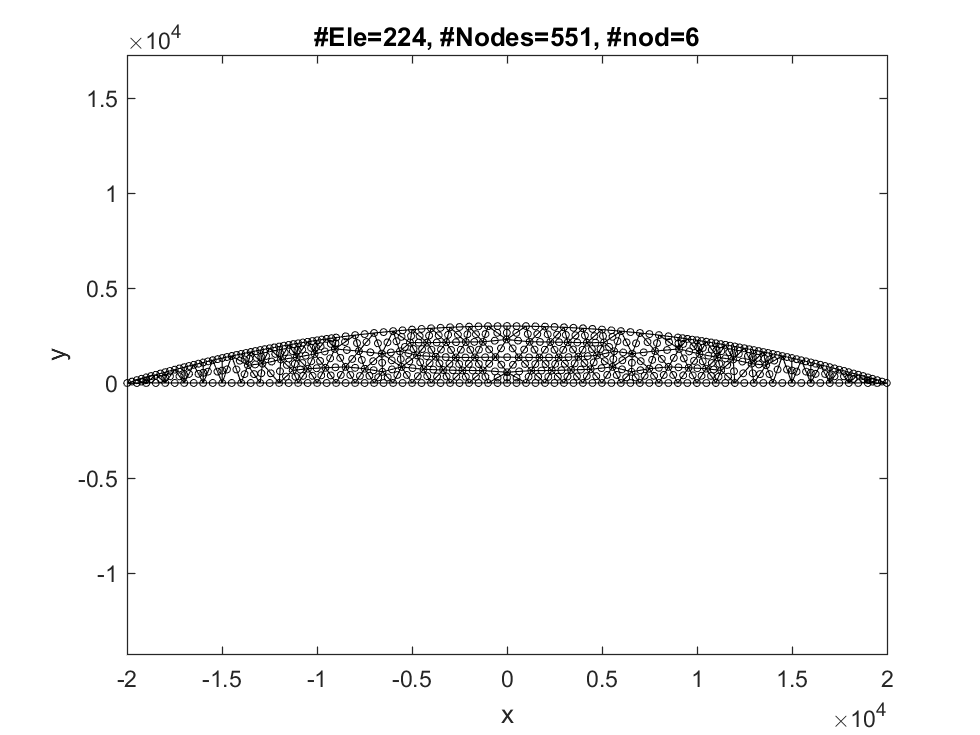
\includegraphics [width=4in]{ExamplesOfMeshGeneration_04.eps}


\subsection*{example:  house withouth a window}

\begin{verbatim}
CtrlVar=Ua2D_DefaultParameters(); CtrlVar.MeshSizeMax=0.1; CtrlVar.MeshSizeMin=0.1;
MeshBoundaryCoordinates=[-1 -1 ; -1 0 ; 0 1 ; 1 0 ; 1 -1 ; 0 -1 ] ;
[MUA,FEmeshTriRep]=genmesh2d(CtrlVar,MeshBoundaryCoordinates); figure ;  PlotFEmesh(MUA.coordinates,MUA.connectivity)
drawnow
%str=input('Next example? y/n [y] ? ','s'); if strcmpi(str,'n') ; return ; end
\end{verbatim}

        \color{lightgray} \begin{verbatim} Creating an input file for gmesh : GmeshFile.geo 
Calling gmesh with GmeshFile.geo as a geo input file, and creating GmeshFile.msh output file 
The gmesh call is:  C:\cygwin64\home\Hilmar\ghg\Ua\gmsh-2.11.0-Windows\gmsh.exe GmeshFile.geo -2 -v 1  
Loading GmeshFile.msh 
 Reading GmeshFile.msh.  
Mesh Type : 2.2 0 8 Reading nodes done.  Reading elements done.
 No inside-out elements. 
  \end{verbatim} \color{black}
    
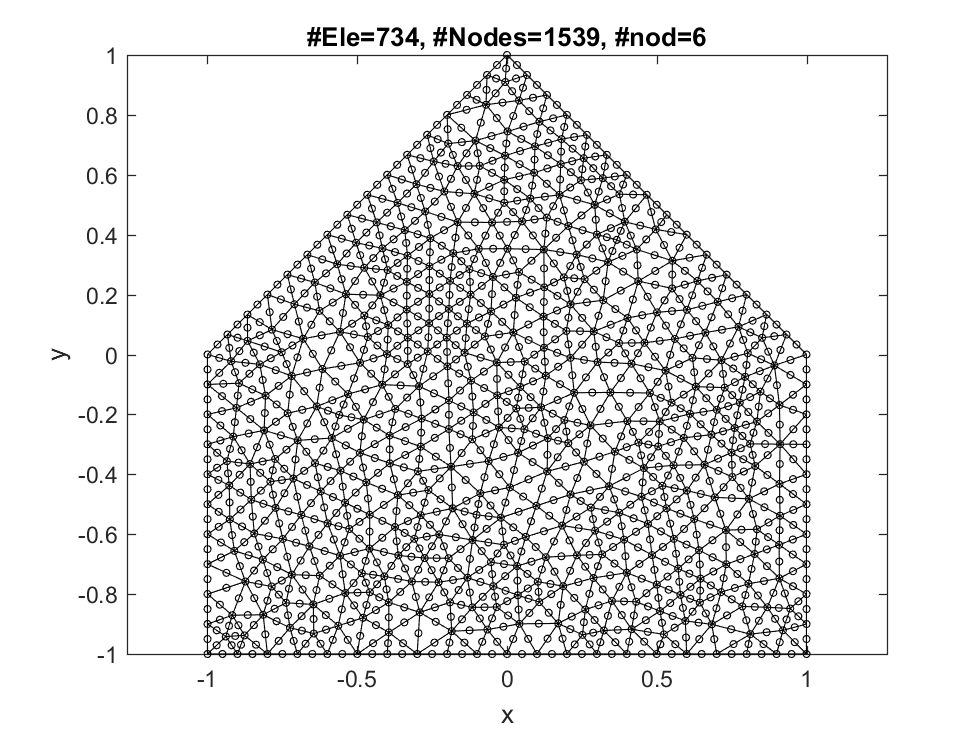
\includegraphics [width=4in]{ExamplesOfMeshGeneration_05.eps}


\subsection*{example: a house with a window! :-)}

\begin{par}
when creating holes within a mesh, separate boundaries by NaN NaN
\end{par} \vspace{1em}
\begin{verbatim}
CtrlVar=Ua2D_DefaultParameters(); CtrlVar.MeshSizeMax=0.1; CtrlVar.MeshSizeMin=0.1;
MeshBoundaryCoordinates=[-1 -1 ; -1 0 ; 0 1 ; 1 0 ; 1 -1 ; 0 -1 ; ...       % Outer boundary (clockwise orientation)
               NaN NaN ;  0.5 -0.5 ; 0.5 0 ; 0.1 0 ; 0.1 -0.5 ; ...         % inner boundary (anticlockwise orientation)
               NaN NaN ; -0.1 -0.5 ; -0.1 0 ; -0.8 0 ; -0.8 -0.5 ];         % another innner boundary (anticlockwise orientation)
[MUA,FEmeshTriRep]=genmesh2d(CtrlVar,MeshBoundaryCoordinates); figure ;  PlotFEmesh(MUA.coordinates,MUA.connectivity)
drawnow
%str=input('Next example? y/n [y] ? ','s'); if strcmpi(str,'n') ; return ; end
\end{verbatim}

        \color{lightgray} \begin{verbatim} Creating an input file for gmesh : GmeshFile.geo 
Calling gmesh with GmeshFile.geo as a geo input file, and creating GmeshFile.msh output file 
The gmesh call is:  C:\cygwin64\home\Hilmar\ghg\Ua\gmsh-2.11.0-Windows\gmsh.exe GmeshFile.geo -2 -v 1  
Loading GmeshFile.msh 
 Reading GmeshFile.msh.  
Mesh Type : 2.2 0 8 Reading nodes done.  Reading elements done.
 No inside-out elements. 
  \end{verbatim} \color{black}
    
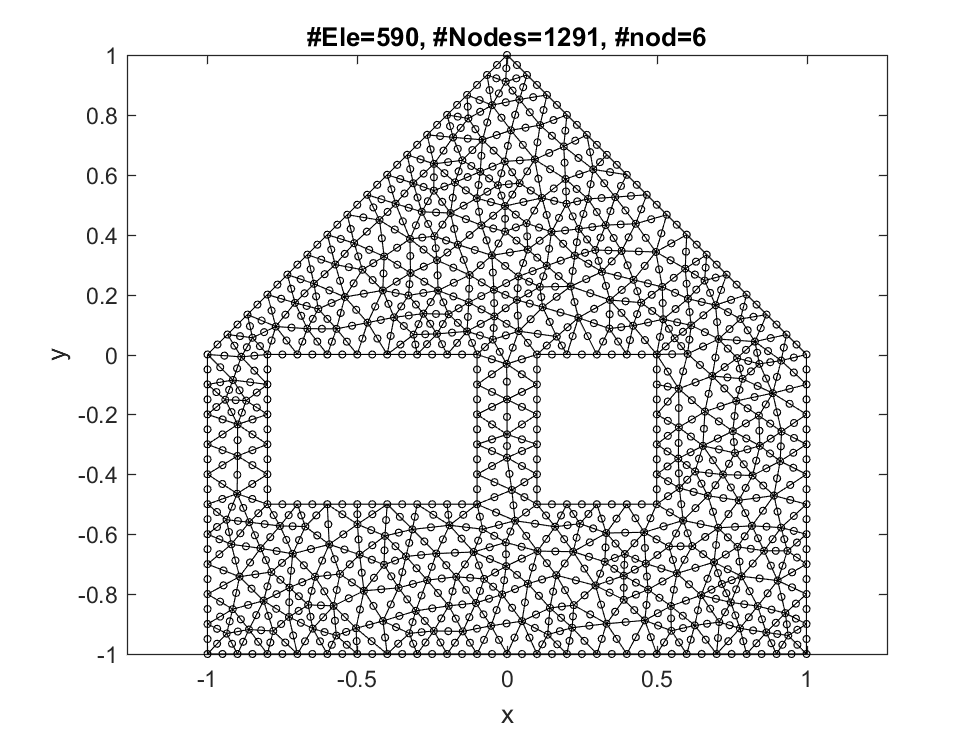
\includegraphics [width=4in]{ExamplesOfMeshGeneration_06.eps}


\subsection*{a house with a tree}

\begin{par}
When generating separate meshed domains, label each domain with a number. The label is the specified by putting `Label NaN' ahead of the corresponding boundary
\end{par} \vspace{1em}
\begin{verbatim}
CtrlVar=Ua2D_DefaultParameters(); CtrlVar.MeshSizeMax=0.1; CtrlVar.MeshSizeMin=0.1;
MeshBoundaryCoordinates=[1 NaN ; -1 -1 ; -1 0 ; 0 1 ; 1 0 ; 1 -1 ; 0 -1 ; ...                                                     % boundary of mesh 1
                         2 NaN ; -2.0 -0.5 ; -2.0 0.5 ; -1.5 0.5 ; -1.5 -0.5 ; -1.7 -0.5 ; -1.7 -1 ; -1.8 -1 ; -1.8 -0.5 ];       % boundary of mesh 2
[MUA,FEmeshTriRep]=genmesh2d(CtrlVar,MeshBoundaryCoordinates); figure ;  PlotFEmesh(MUA.coordinates,MUA.connectivity)

drawnow
%str=input('Next example? y/n [y] ? ','s'); if strcmpi(str,'n') ; return ; end
\end{verbatim}

        \color{lightgray} \begin{verbatim} Creating an input file for gmesh : GmeshFile.geo 
Calling gmesh with GmeshFile.geo as a geo input file, and creating GmeshFile.msh output file 
The gmesh call is:  C:\cygwin64\home\Hilmar\ghg\Ua\gmsh-2.11.0-Windows\gmsh.exe GmeshFile.geo -2 -v 1  
Loading GmeshFile.msh 
 Reading GmeshFile.msh.  
Mesh Type : 2.2 0 8 Reading nodes done.  Reading elements done.
 No inside-out elements. 
  \end{verbatim} \color{black}
    
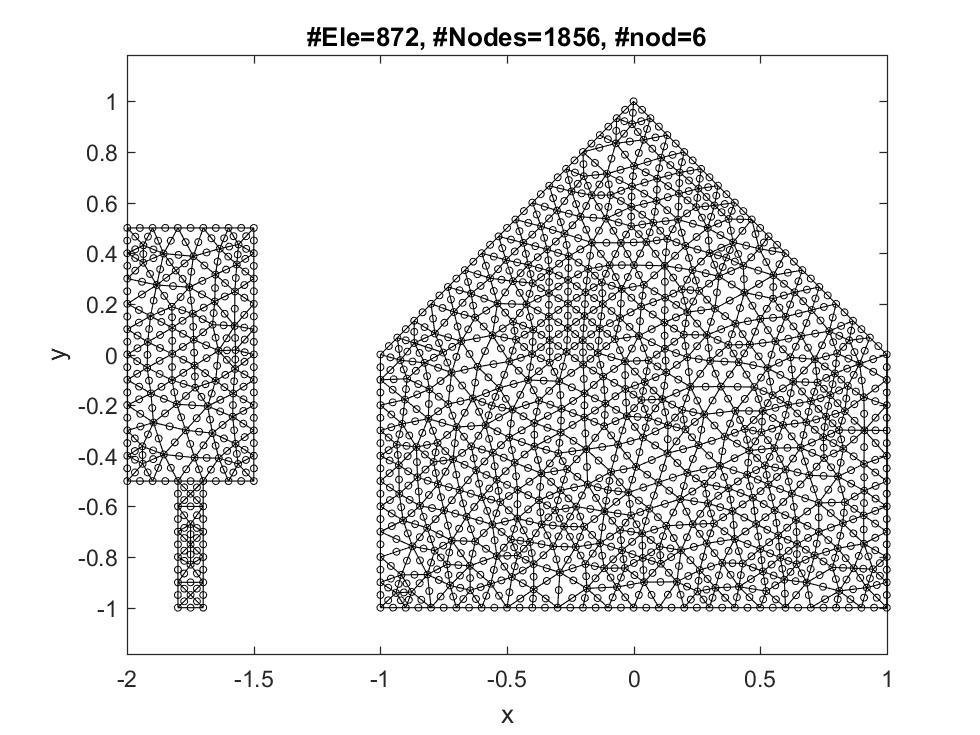
\includegraphics [width=4in]{ExamplesOfMeshGeneration_07.eps}


\subsection*{a house with windows and a tree}

\begin{par}
When generating several separate meshed domains with holes, make sure to specify the outer boundary first, then the holes, and indicate to which mesh a given boundary belongs
\end{par} \vspace{1em}
\begin{verbatim}
CtrlVar=Ua2D_DefaultParameters(); CtrlVar.MeshSizeMax=0.1; CtrlVar.MeshSizeMin=0.1;
MeshBoundaryCoordinates=[1 NaN ; -1 -1 ; -1 0 ; 0 1 ; 1 0 ; 1 -1 ; 0 -1 ; ...      % outer boundary of mesh 1 (clockwise)
    1 NaN ; 0.5 -0.5 ; 0.5 0 ; 0.1 0 ; 0.1 -0.5 ; ...                              % a hole within mesh 1     (anticlockwise)
    1 NaN ; -0.1 -0.5 ; -0.1 0 ; -0.8 0 ; -0.8 -0.5 ; ...                          % a further hole within mesh 1 (anticlockwise)
    3 NaN ; -2.0 -0.5 ; -2.0 0.5 ; -1.5 0.5 ; -1.5 -0.5 ; -1.7 -0.5 ; -1.7 -1 ; -1.8 -1 ; -1.8 -0.5 ];   % another mesh (clockwise). mesh labels do not need to be in sequential order
[MUA,FEmeshTriRep]=genmesh2d(CtrlVar,MeshBoundaryCoordinates); figure ;  PlotFEmesh(MUA.coordinates,MUA.connectivity)
drawnow
%str=input('Next example? y/n [y] ? ','s'); if strcmpi(str,'n') ; return ; end
\end{verbatim}

        \color{lightgray} \begin{verbatim} Creating an input file for gmesh : GmeshFile.geo 
Calling gmesh with GmeshFile.geo as a geo input file, and creating GmeshFile.msh output file 
The gmesh call is:  C:\cygwin64\home\Hilmar\ghg\Ua\gmsh-2.11.0-Windows\gmsh.exe GmeshFile.geo -2 -v 1  
Loading GmeshFile.msh 
 Reading GmeshFile.msh.  
Mesh Type : 2.2 0 8 Reading nodes done.  Reading elements done.
 No inside-out elements. 
  \end{verbatim} \color{black}
    
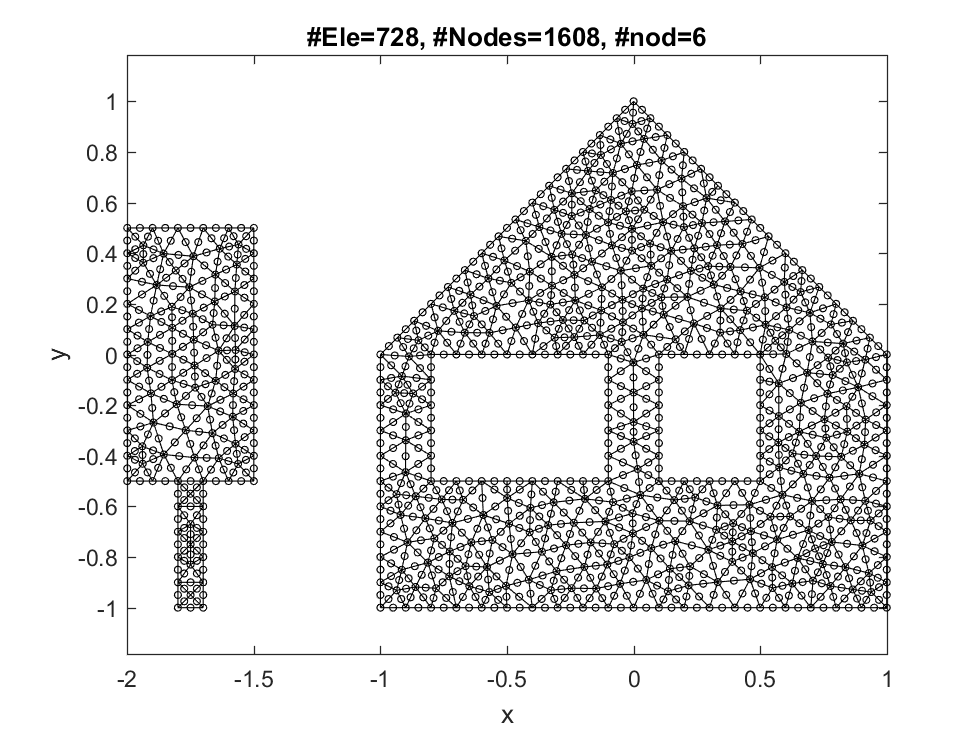
\includegraphics [width=4in]{ExamplesOfMeshGeneration_08.eps}


\subsection*{mesh with several holes and islands}

\begin{verbatim}
CtrlVar=Ua2D_DefaultParameters(); CtrlVar.MeshSizeMax=0.1; CtrlVar.MeshSizeMin=0.1; CtrlVar.TriNodes=10 ;
MeshBoundaryCoordinates=...
    [1 NaN ; -1 -1 ; -1 0 ; 0 1 ; 1 0 ; 1 -1 ; 0 -1 ; ...     % outer boundary of mesh 1
    1 NaN ; 0.5 -0.5 ; 0.5 0 ; 0.1 0 ; 0.1 -0.5 ; ...         % inner boundary of mesh 1
    1 NaN ; -0.1 -0.5 ; -0.1 0 ; -0.8 0 ; -0.8 -0.5 ; ...     % another inner boundary of mesh 1
    2 NaN ; -0.7 -0.4 ; -0.7 -0.1 ; -0.2 -0.1 ; -0.2 -0.4 ; ...   % outer boundary of mesh 2
    40 NaN ; -3.0 -1.0 ; -3.0  0.5 ; -1.5 0.5 ; -1.5 -1.0 ;...    % outer boundary of mesh 40
    40 NaN ; -2.8 -0.8 ; -1.8 -0.8 ; -1.8 0.4 ; -2.8  0.4 ; ...   % inner boundary of mesh 40
    50 NaN ; -2.6 -0.6 ; -2.6 0.3 ; -2.0 0.3 ; -2.0 -0.6  ; ...   % outer boundary of mesh 50
    50 NaN ; -2.5 -0.5 ; -2.1 -0.5 ; -2.1 0.1 ; -2.5 0.1 ];       % inner boundary of mesh 50

CtrlVar.GmeshMeshingAlgorithm=8;    % see gmsh manual


[MUA,FEmeshTriRep]=genmesh2d(CtrlVar,MeshBoundaryCoordinates); figure ;  PlotFEmesh(MUA.coordinates,MUA.connectivity)

% also calculate and plot normals
[nx,ny,xn,yn,Nx,Ny] = CalcEdgeAndNodalNormals(MUA.connectivity,MUA.coordinates,MUA.Boundary.Edges);
QuiverColorGHG(MUA.coordinates(MUA.Boundary.Nodes,1),MUA.coordinates(MUA.Boundary.Nodes,2),...
     Nx(MUA.Boundary.Nodes),Ny(MUA.Boundary.Nodes),[]);
drawnow

 %str=input('Next example? y/n [y] ? ','s'); if strcmpi(str,'n') ; return ; end
\end{verbatim}

        \color{lightgray} \begin{verbatim} Creating an input file for gmesh : GmeshFile.geo 
Calling gmesh with GmeshFile.geo as a geo input file, and creating GmeshFile.msh output file 
The gmesh call is:  C:\cygwin64\home\Hilmar\ghg\Ua\gmsh-2.11.0-Windows\gmsh.exe GmeshFile.geo -2 -v 1  
Loading GmeshFile.msh 
 Reading GmeshFile.msh.  
Mesh Type : 2.2 0 8 Reading nodes done.  Reading elements done.
 No inside-out elements. 
  QuiverColorGHG: uvPlotScale=15.000000 
\end{verbatim} \color{black}
    
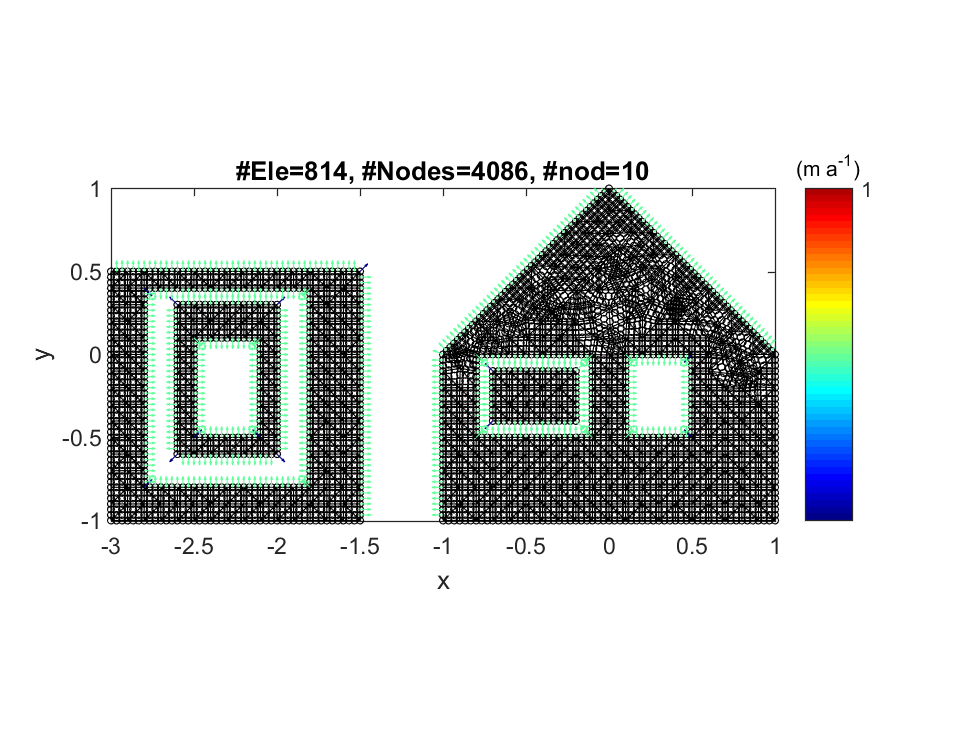
\includegraphics [width=4in]{ExamplesOfMeshGeneration_09.eps}
\begin{par}
Example: a constrainted meshing with two joined meshes sharing the same boundary
\end{par} \vspace{1em}
\begin{par}
Since here the same line belongs to more then one mesh we need to specify the 'plane surface' (gmsh terminology) separatly. This is done in CtrlVar.GmshPlaneSurface
\end{par} \vspace{1em}
\begin{verbatim}
CtrlVar=Ua2D_DefaultParameters(); CtrlVar.MeshSizeMax=0.1; CtrlVar.MeshSizeMin=0.1;
MeshBoundaryCoordinates=[1 NaN ;-1 -1 ; -1 0 ; 0 1 ; 1 0 ; 1 -1 ; 0 -1 ; ...       % Outer boundary (clockwise orientation)
                         1 NaN ;  0.5 -0.5 ; 0.5 0 ; 0.1 0 ; 0.1 -0.5 ; ...         % inner boundary (anticlockwise orientation)
                         1 NaN ; -0.1 -0.5 ; 0 0.3 ; -0.95 0 ; -0.8 -0.9 ];         % another innner boundary (anticlockwise orientation)

CtrlVar.GmshPlaneSurface{1}=[1 2 3]; % mesh 1 is defined by boundaries 1, 2 and 3
CtrlVar.GmshPlaneSurface{2}=[-2];  % mesh 2 is defined by boundary 2, make sure to use a negative sign to indicate a reverse ordering
CtrlVar.GmshPlaneSurface{3}=[-3];  % mesh 2 is defined by boundary 2, make sure to use a negative sign to indicate a reverse ordering
[MUA,FEmeshTriRep]=genmesh2d(CtrlVar,MeshBoundaryCoordinates); figure ;  PlotFEmesh(MUA.coordinates,MUA.connectivity)

plot(MeshBoundaryCoordinates(:,1),MeshBoundaryCoordinates(:,2),'-or','LineWidth',2)

drawnow
%str=input('Next example? y/n [y] ? ','s'); if strcmpi(str,'n') ; return ; end
\end{verbatim}

        \color{lightgray} \begin{verbatim} Creating an input file for gmesh : GmeshFile.geo 
Calling gmesh with GmeshFile.geo as a geo input file, and creating GmeshFile.msh output file 
The gmesh call is:  C:\cygwin64\home\Hilmar\ghg\Ua\gmsh-2.11.0-Windows\gmsh.exe GmeshFile.geo -2 -v 1  
Loading GmeshFile.msh 
 Reading GmeshFile.msh.  
Mesh Type : 2.2 0 8 Reading nodes done.  Reading elements done.
 No inside-out elements. 
  \end{verbatim} \color{black}
    
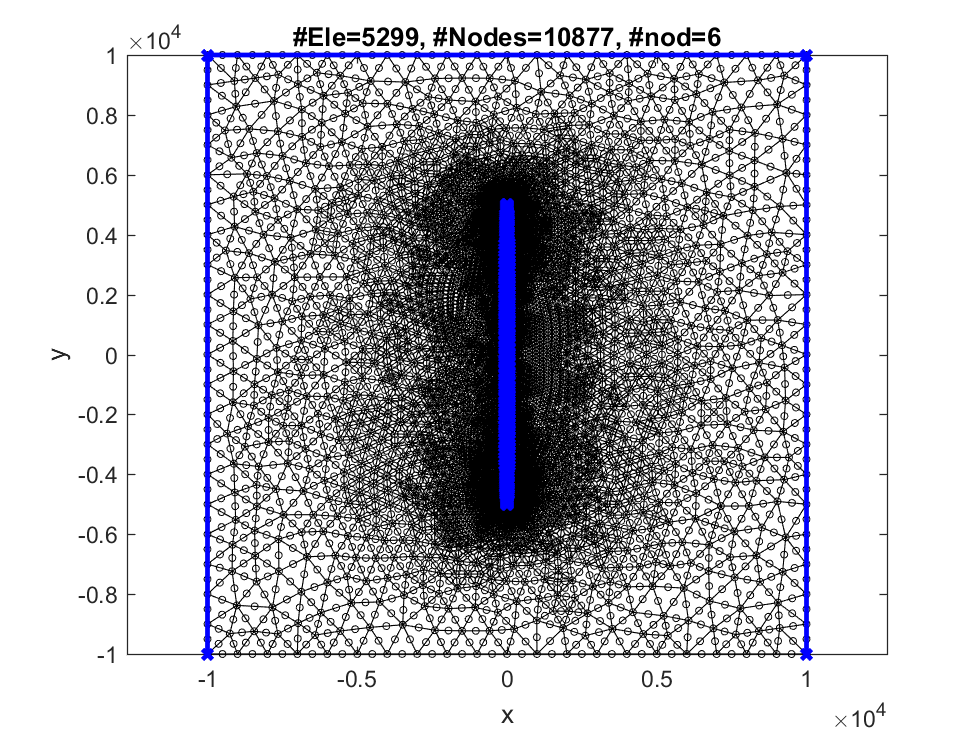
\includegraphics [width=4in]{ExamplesOfMeshGeneration_10.eps}
\begin{par}
example: two separate meshes in contact
\end{par} \vspace{1em}
\begin{verbatim}
CtrlVar=Ua2D_DefaultParameters(); CtrlVar.MeshSizeMax=0.1; CtrlVar.MeshSizeMin=0.1;
MeshBoundaryCoordinates=[1 NaN ;  0 0  ; 0 1 ; 1 1 ; 1 0 ; ...
                         2 NaN ; -1 0  ; -1 1.001 ; 0 1.001 ; 0 0 ];

[MUA,FEmeshTriRep]=genmesh2d(CtrlVar,MeshBoundaryCoordinates); figure ;  PlotFEmesh(MUA.coordinates,MUA.connectivity)

plot(MeshBoundaryCoordinates(:,1),MeshBoundaryCoordinates(:,2),'-or','LineWidth',2)
drawnow
%str=input('Next example? y/n [y] ? ','s'); if strcmpi(str,'n') ; return ; end
\end{verbatim}

        \color{lightgray} \begin{verbatim} Creating an input file for gmesh : GmeshFile.geo 
Calling gmesh with GmeshFile.geo as a geo input file, and creating GmeshFile.msh output file 
The gmesh call is:  C:\cygwin64\home\Hilmar\ghg\Ua\gmsh-2.11.0-Windows\gmsh.exe GmeshFile.geo -2 -v 1  
Loading GmeshFile.msh 
 Reading GmeshFile.msh.  
Mesh Type : 2.2 0 8 Reading nodes done.  Reading elements done.
 No inside-out elements. 
  \end{verbatim} \color{black}
    
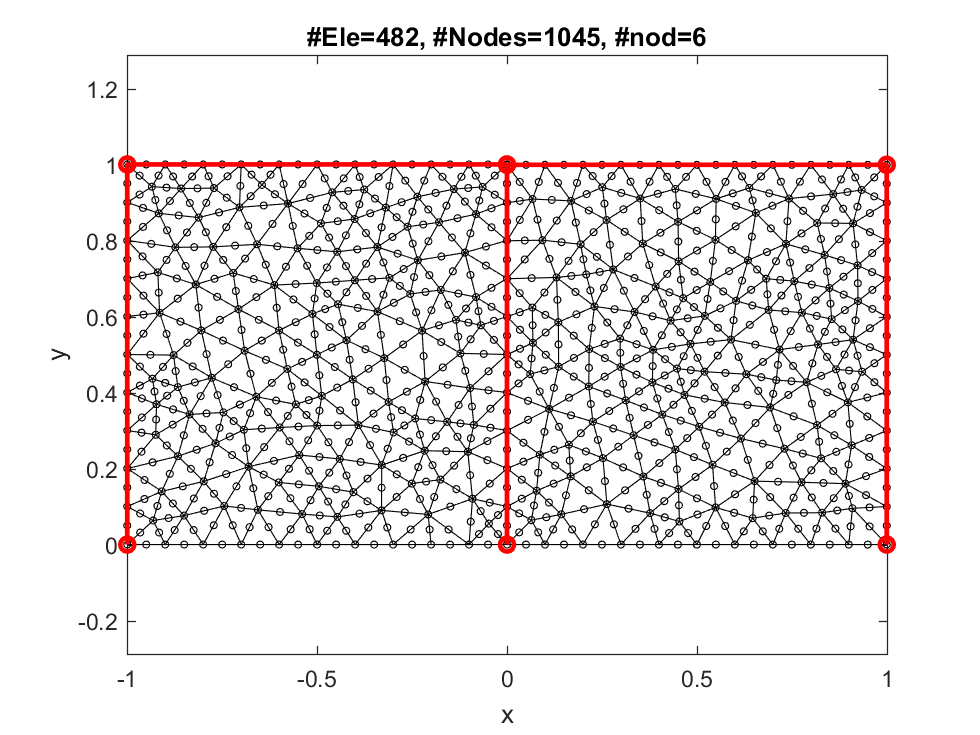
\includegraphics [width=4in]{ExamplesOfMeshGeneration_11.eps}
\begin{par}
example: two separate meshes in contact
\end{par} \vspace{1em}
\begin{verbatim}
CtrlVar=Ua2D_DefaultParameters(); CtrlVar.MeshSizeMax=0.1; CtrlVar.MeshSizeMin=0.1; CtrlVar.GmshInputFormat=1;
MeshBoundaryCoordinates=[1 NaN ;  0 0  ; 0 0.25 ; 0.25 0.25 ; 0.25 0.75 ; 0 0.75 ; 0 1 ; 1 1 ; 1 0;   ...
                         2 NaN ;  0 0.25 ; 0. 0.75 ; 0.25 0.75 ; 0.25 0.25 ];

[MUA,FEmeshTriRep]=genmesh2d(CtrlVar,MeshBoundaryCoordinates);
figure ;  PlotFEmesh(MUA.coordinates,MUA.connectivity)

plot(MeshBoundaryCoordinates(:,1),MeshBoundaryCoordinates(:,2),'-or','LineWidth',2)
drawnow
%str=input('Next example? y/n [y] ? ','s');  if strcmpi(str,'n') ; return ; end
\end{verbatim}

        \color{lightgray} \begin{verbatim} Creating an input file for gmesh : GmeshFile.geo 
Calling gmesh with GmeshFile.geo as a geo input file, and creating GmeshFile.msh output file 
The gmesh call is:  C:\cygwin64\home\Hilmar\ghg\Ua\gmsh-2.11.0-Windows\gmsh.exe GmeshFile.geo -2 -v 1  
Loading GmeshFile.msh 
 Reading GmeshFile.msh.  
Mesh Type : 2.2 0 8 Reading nodes done.  Reading elements done.
 No inside-out elements. 
  \end{verbatim} \color{black}
    
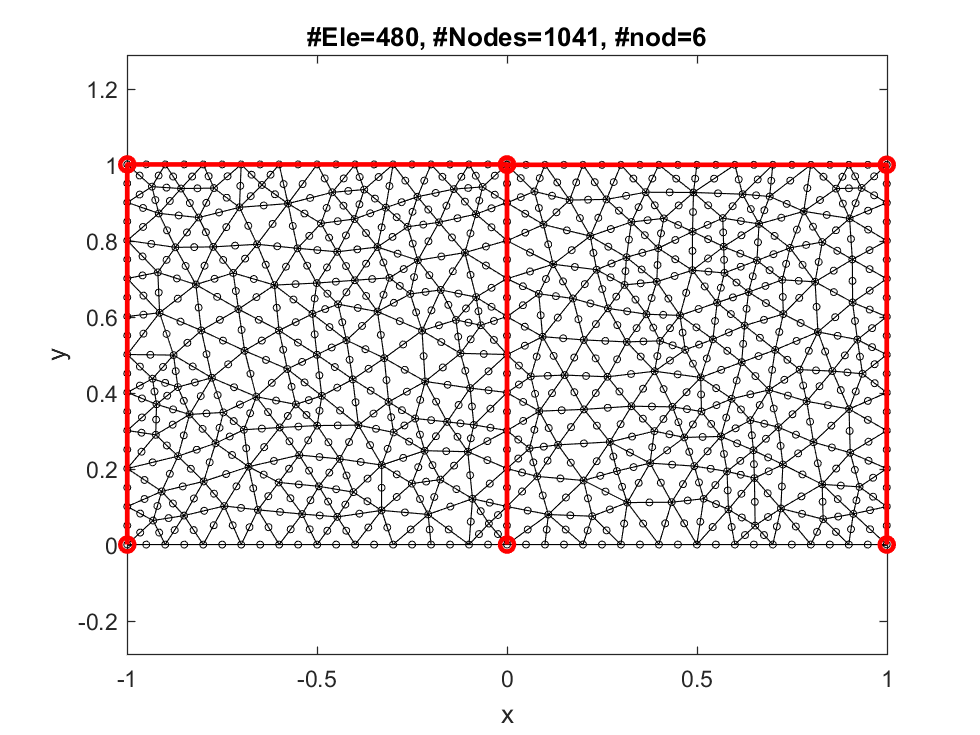
\includegraphics [width=4in]{ExamplesOfMeshGeneration_12.eps}
\begin{par}
Example: Two subdomains sharing a common boundary.
\end{par} \vspace{1em}
\begin{par}
This example uses GmshInputFormat 2.
\end{par} \vspace{1em}
\begin{par}
Gmsh input format 2 is quite close to the gmsh input format itself and more flexible than the default input format 1, but also more difficult to use.
\end{par} \vspace{1em}
\begin{par}
The gmsh input format 2 does not use `MeshBoundaryCoordinates' at all.
\end{par} \vspace{1em}
\begin{par}
Using gmsh input format 2 allows constraint meshing. The computational domain can be split up into several subdomains. each with their own boundaries. One can create internal boundaries within a domain, and subdomains sharing some common boundaries.
\end{par} \vspace{1em}
\begin{par}
All inputs are defined as fields to the CtrlVar.
\end{par} \vspace{1em}
\begin{par}
The basic idea is to define points, then to specify lines in terms of those points, loops in terms of those lines, and finally plane surfaces in terms of the loops.
\end{par} \vspace{1em}
\begin{verbatim}
CtrlVar=Ua2D_DefaultParameters();

CtrlVar.GmshInputFormat=2; % using input format 2
CtrlVar.MeshSizeMax=0.1;
CtrlVar.MeshSizeMin=0.1;
CtrlVar.MeshSize=0.1;

CtrlVar.Gmsh.Points=[0 0 ;...    % now define a few gmsh points
                     0 0.5 ; ... % although not directly labeled
                     0 1 ;   ... % the first point in point 1, etc.
                     1 1 ;  ...
                     1 0 ; ...
                     -1 0 ; ...   % this is point nr 5
                     -1 0.5];     % and this point nr 7

CtrlVar.Gmsh.Lines{1}=[1 , 2];  % define gmsh lines using the point labels
CtrlVar.Gmsh.Lines{2}=[2 , 3];
CtrlVar.Gmsh.Lines{3}=[ 3 ; 4 ; 5 ; 1 ];
CtrlVar.Gmsh.Lines{4}=[ 1 ;  6 ; 7 ; 2 ];

CtrlVar.Gmsh.Loops{1}=[1 ; 2 ; 3 ]; % now define loops
CtrlVar.Gmsh.Loops{2}=[4 ; -1];     % all loops must be closed!

CtrlVar.Gmsh.PlaneSurfaces{1} = [1]; % finally define the surfaces
CtrlVar.Gmsh.PlaneSurfaces{2} = [2];

MeshBoundaryCoordinates=[]; % When CtrlVar.GmshInputFormat=2, 'MeshBoundaryCoordinates' are not used
[MUA,FEmeshTriRep]=genmesh2d(CtrlVar,MeshBoundaryCoordinates);
figure ;  PlotFEmesh(MUA.coordinates,MUA.connectivity)
hold on ; PlotGmshGeometryDefinition(CtrlVar);
drawnow
%str=input('Next example? y/n [y] ? ','s');  if strcmpi(str,'n') ; return ; end
\end{verbatim}

        \color{lightgray} \begin{verbatim} Creating an input file for gmesh : GmeshFile.geo 
Calling gmesh with GmeshFile.geo as a geo input file, and creating GmeshFile.msh output file 
The gmesh call is:  C:\cygwin64\home\Hilmar\ghg\Ua\gmsh-2.11.0-Windows\gmsh.exe GmeshFile.geo -2 -v 1  
Loading GmeshFile.msh 
 Reading GmeshFile.msh.  
Mesh Type : 2.2 0 8 Reading nodes done.  Reading elements done.
 No inside-out elements. 
  \end{verbatim} \color{black}
    
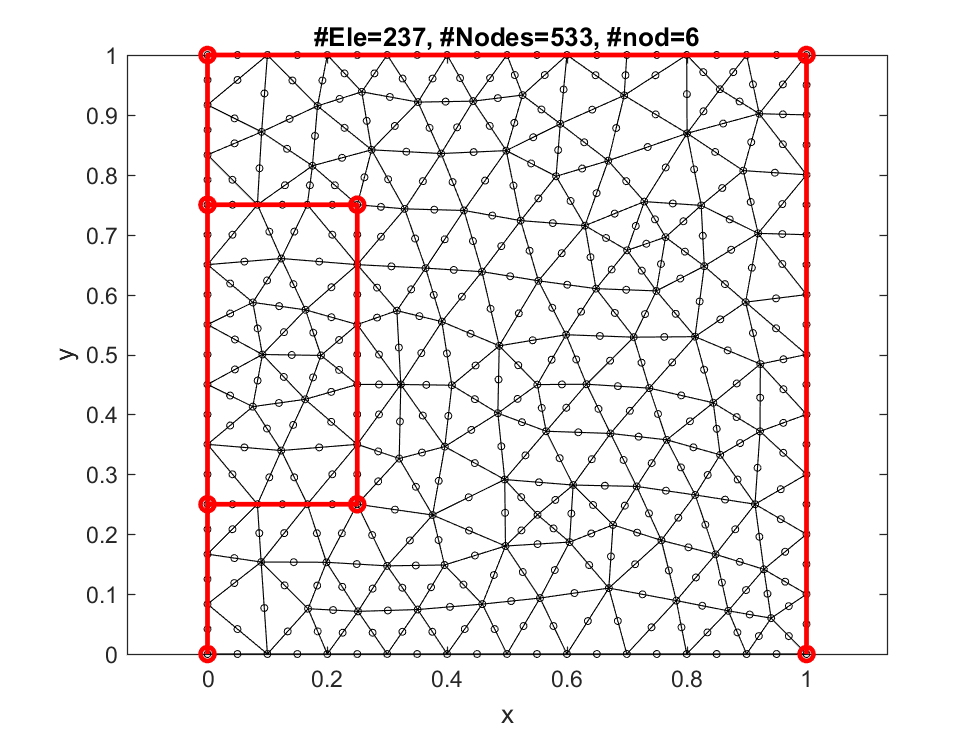
\includegraphics [width=4in]{ExamplesOfMeshGeneration_13.eps}
\begin{par}
Example: Several different subdomains, internal domain, separated domains, joined-up domains.
\end{par} \vspace{1em}
\begin{par}
This example uses gmsh input format 2
\end{par} \vspace{1em}
\begin{verbatim}
CtrlVar=Ua2D_DefaultParameters();
MeshBoundaryCoordinates=[];
CtrlVar.GmshInputFormat=2;
CtrlVar.MeshSizeMax=0.1; CtrlVar.MeshSizeMin=0.1; CtrlVar.TriNodes=3;

CtrlVar.Gmsh.Points=[0 0 ;...
                     0 0.5 ; ...
                     0 1 ;   ...
                     1 1 ;  ...
                     1 0 ; ...
                     -1 0 ; ...
                     -1 0.5 ; ...
                     0.25 0.25 ; ...
                     0.35 0.75 ; ...
                     0.65 0.75 ;
                     0.80 0.25 ;
                     -0.5 1 ; ...
                     -1 2 ; ...
                     1 2 ; ...
                     ];

CtrlVar.Gmsh.Lines{1}=[1 ; 2];
CtrlVar.Gmsh.Lines{2}=[2 ; 3];
CtrlVar.Gmsh.Lines{3}=[ 3 ; 4 ; 5 ; 1 ];
CtrlVar.Gmsh.Lines{4}=[ 1 ;  6 ; 7 ; 2 ];
CtrlVar.Gmsh.Lines{5}=[ 8 ; 9 ; 10 ; 11 ; 8];
CtrlVar.Gmsh.Lines{6}=[ 12 ; 13 ; 14 ; 12];

CtrlVar.Gmsh.Loops{1}=[1 ; 2 ; 3 ];
CtrlVar.Gmsh.Loops{2}=[4 ; -1];
CtrlVar.Gmsh.Loops{3}=[-5]; % reverse orientation
CtrlVar.Gmsh.Loops{4}=[6];
CtrlVar.Gmsh.Loops{5}=[5];  %

CtrlVar.Gmsh.PlaneSurfaces{1} = [1 ; 3 ]; % this surface has a hole
CtrlVar.Gmsh.PlaneSurfaces{2} = [2];
CtrlVar.Gmsh.PlaneSurfaces{3} = [4];
CtrlVar.Gmsh.PlaneSurfaces{4} = [5];


MUA=genmesh2d(CtrlVar,MeshBoundaryCoordinates);

% plotting mesh
figure ;  PlotFEmesh(MUA.coordinates,MUA.connectivity)
hold on
PlotGmshGeometryDefinition(CtrlVar);

drawnow
%str=input('Next example? y/n [y] ? ','s');  if strcmpi(str,'n') ; return ; end
\end{verbatim}

        \color{lightgray} \begin{verbatim} Creating an input file for gmesh : GmeshFile.geo 
Calling gmesh with GmeshFile.geo as a geo input file, and creating GmeshFile.msh output file 
The gmesh call is:  C:\cygwin64\home\Hilmar\ghg\Ua\gmsh-2.11.0-Windows\gmsh.exe GmeshFile.geo -2 -v 1  
Loading GmeshFile.msh 
 Reading GmeshFile.msh.  
Mesh Type : 2.2 0 8 Reading nodes done.  Reading elements done.
 No inside-out elements. 
  \end{verbatim} \color{black}
    
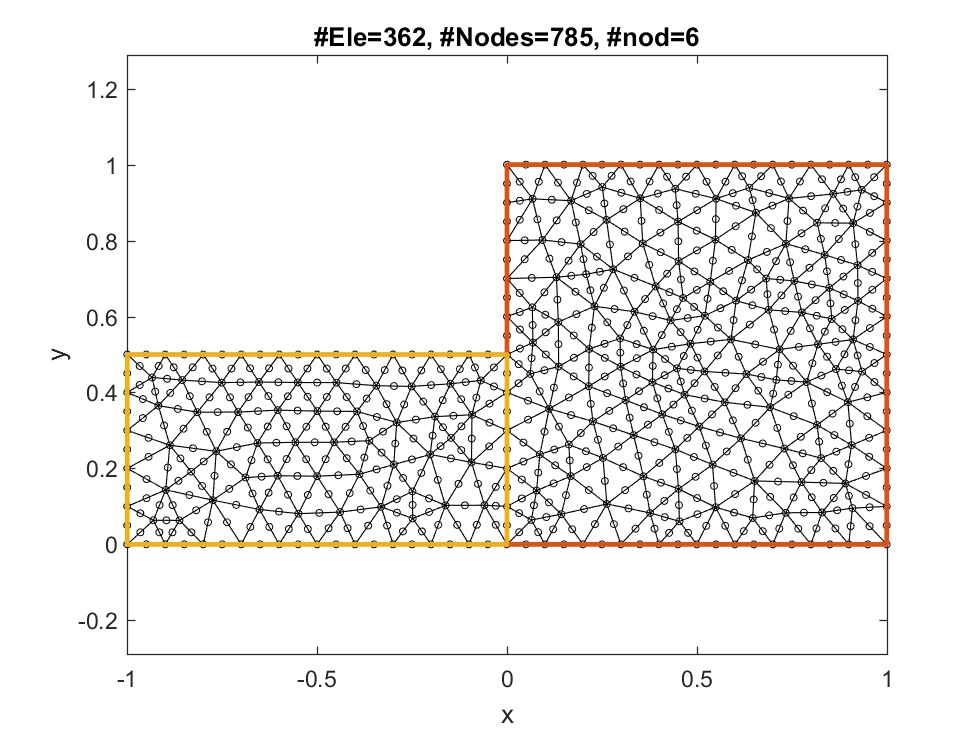
\includegraphics [width=4in]{ExamplesOfMeshGeneration_14.eps}
\begin{par}
Example: Meshing the Brunt Ice Shelf
\end{par} \vspace{1em}
\begin{verbatim}
load BruntMeshBoundaryCoordinates.mat

I=find(isnan(MeshBoundaryCoordinates(:,1)) | isnan(MeshBoundaryCoordinates(:,2)));

i1a=I(1)+1 ; i1b=I(2)-1;
i2a=I(2)+1 ; i2b=size(MeshBoundaryCoordinates,1);


CtrlVar=Ua2D_DefaultParameters();
CtrlVar.GmshInputFormat=2;
CtrlVar.MeshSizeMax=5e3;
CtrlVar.MeshSizeMin=1e3;
CtrlVar.TriNodes=3;


CtrlVar.Gmsh.Points=MeshBoundaryCoordinates(i1a:i1b,:);

CtrlVar.Gmsh.Loops{1}=[1];
CtrlVar.Gmsh.PlaneSurfaces{1} = [1];
CtrlVar.Gmsh.Lines{1}=[(1:i1b-i1a+1)';1];
MUA=genmesh2d(CtrlVar,MeshBoundaryCoordinates);


% plotting mesh
figure ;  PlotFEmesh(MUA.coordinates,MUA.connectivity)
drawnow
%str=input('Next example? y/n [y] ? ','s');  if strcmpi(str,'n') ; return ; end
\end{verbatim}

        \color{lightgray} \begin{verbatim} Creating an input file for gmesh : GmeshFile.geo 
Calling gmesh with GmeshFile.geo as a geo input file, and creating GmeshFile.msh output file 
The gmesh call is:  C:\cygwin64\home\Hilmar\ghg\Ua\gmsh-2.11.0-Windows\gmsh.exe GmeshFile.geo -2 -v 1  
Loading GmeshFile.msh 
 Reading GmeshFile.msh.  
Mesh Type : 2.2 0 8 Reading nodes done.  Reading elements done.
 No inside-out elements. 
  \end{verbatim} \color{black}
    
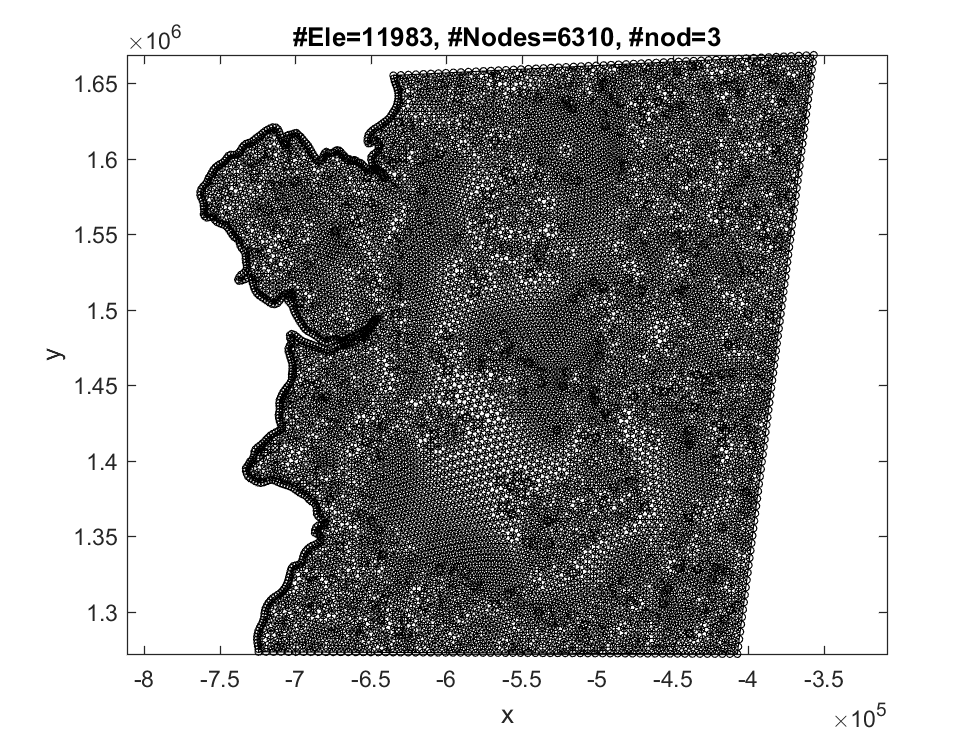
\includegraphics [width=4in]{ExamplesOfMeshGeneration_15.eps}
\begin{par}
Example: Meshing the Brunt Ice Shelf with an internal boundary
\end{par} \vspace{1em}
\begin{verbatim}
load BruntMeshBoundaryCoordinates.mat
CtrlVar.Gmsh.Points=[MeshBoundaryCoordinates(i1a:i1b,:); MeshBoundaryCoordinates(i2a:i2b,:) ];
l1a=1 ; l1b=l1a+i1b-i1a;
l2a=l1b+1 ; l2b=l2a+i2b-i2a;
CtrlVar.Gmsh.Lines{1}=[(l1a:l1b)';l1a];
CtrlVar.Gmsh.Lines{2}=[(l2a:l2b)';l2a];
CtrlVar.Gmsh.Loops{1}=[1];
CtrlVar.Gmsh.Loops{2}=[2];
CtrlVar.Gmsh.PlaneSurfaces{1} = [1,-2];
CtrlVar.Gmsh.PlaneSurfaces{2} = [2];


MUA=genmesh2d(CtrlVar,MeshBoundaryCoordinates);
CtrlVar.Gmsh.Lines{1}=[(1:i1b-i1a+1)';1];

% plotting mesh
figure ;  PlotFEmesh(MUA.coordinates,MUA.connectivity)

hold on ; PlotGmshGeometryDefinition(CtrlVar);
drawnow
%str=input('Next example? y/n [y] ? ','s');  if strcmpi(str,'n') ; return ; end
\end{verbatim}

        \color{lightgray} \begin{verbatim} Creating an input file for gmesh : GmeshFile.geo 
Calling gmesh with GmeshFile.geo as a geo input file, and creating GmeshFile.msh output file 
The gmesh call is:  C:\cygwin64\home\Hilmar\ghg\Ua\gmsh-2.11.0-Windows\gmsh.exe GmeshFile.geo -2 -v 1  
Loading GmeshFile.msh 
 Reading GmeshFile.msh.  
Mesh Type : 2.2 0 8 Reading nodes done.  Reading elements done.
 No inside-out elements. 
  \end{verbatim} \color{black}
    
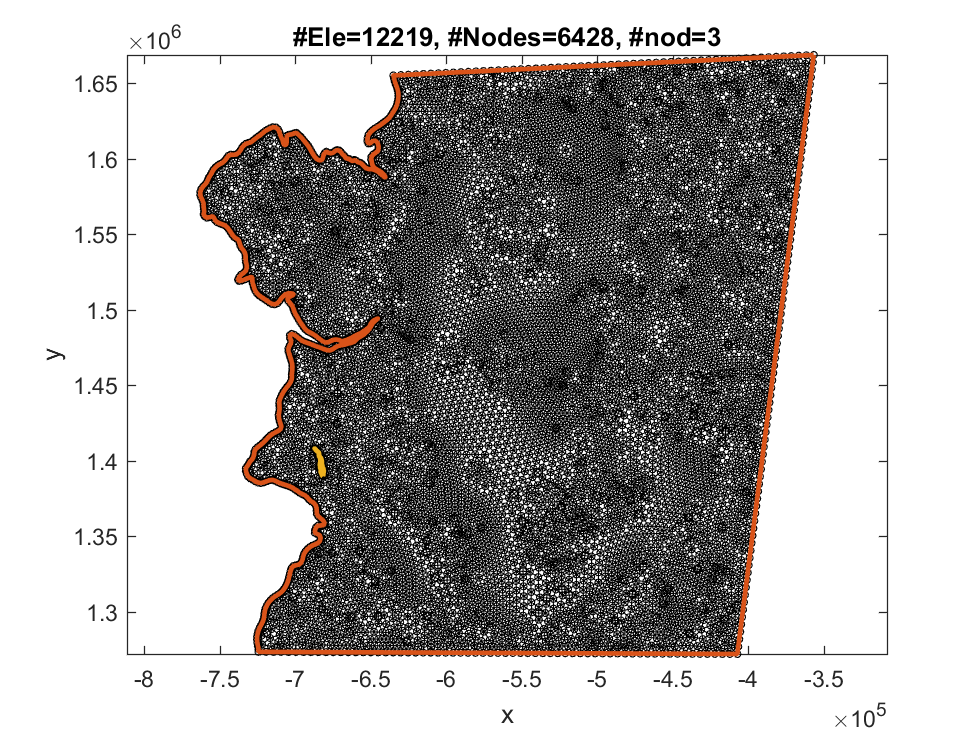
\includegraphics [width=4in]{ExamplesOfMeshGeneration_16.eps}
\begin{par}
Example: Meshing the Brunt Ice Shelf with an internal boundary and a `fill-in'
\end{par} \vspace{1em}
\begin{verbatim}
load BruntMeshBoundaryCoordinates.mat

I=find(isnan(MeshBoundaryCoordinates(:,1)) | isnan(MeshBoundaryCoordinates(:,2)));

i1a=I(1)+1 ; i1b=I(2)-1;
i2a=I(2)+1 ; i2b=size(MeshBoundaryCoordinates,1);


CtrlVar=Ua2D_DefaultParameters();
CtrlVar.GmshInputFormat=2;
CtrlVar.MeshSizeMax=5e3;
CtrlVar.MeshSizeMin=1e3;
CtrlVar.TriNodes=3;
CtrlVar.Gmsh.Points=[MeshBoundaryCoordinates(i1a:i1b,:); MeshBoundaryCoordinates(i2a:i2b,:) ];
l1a=1 ; l1b=l1a+i1b-i1a;
l2a=l1b+1 ; l2b=l2a+i2b-i2a;
CtrlVar.Gmsh.Lines{1}=[(l1a:l1b)';l1a];
CtrlVar.Gmsh.Lines{2}=[(l2a:l2b)';l2a];


Box=[-7.02e+05  -6.4314e+05   1.4651e+06   1.505e+06];
I=CtrlVar.Gmsh.Points(:,1) > Box(1) & CtrlVar.Gmsh.Points(:,1) < Box(2) ...
    & CtrlVar.Gmsh.Points(:,2) > Box(3) & CtrlVar.Gmsh.Points(:,2) < Box(4) ;

% now must line 1 into two lines, with one convering the BIS-SW chasm outlines only

x=CtrlVar.Gmsh.Points(CtrlVar.Gmsh.Lines{1},1);
y=CtrlVar.Gmsh.Points(CtrlVar.Gmsh.Lines{1},2);
K=x > Box(1) & x < Box(2) ...
    & y > Box(3) & y < Box(4) ;

temp=CtrlVar.Gmsh.Lines{1};
temp(K)=NaN; temp(end)=[];
J=find(isnan(temp));
tt=[temp(J(end)+1:end,end);temp(1:J(1)-1)];
CtrlVar.Gmsh.Lines{3}=tt;
CtrlVar.Gmsh.Lines{4}=find(K);
CtrlVar.Gmsh.Lines{4}=[CtrlVar.Gmsh.Lines{3}(end); CtrlVar.Gmsh.Lines{4};CtrlVar.Gmsh.Lines{3}(1)];

CtrlVar.Gmsh.Lines{5}=[CtrlVar.Gmsh.Lines{3}(end);CtrlVar.Gmsh.Lines{3}(1)];
CtrlVar.Gmsh.Lines{6}=[CtrlVar.Gmsh.Lines{4}(end);CtrlVar.Gmsh.Lines{4}(1)];

figure
plot(CtrlVar.Gmsh.Points(CtrlVar.Gmsh.Lines{1},1),CtrlVar.Gmsh.Points(CtrlVar.Gmsh.Lines{1},2),'.-')
hold on
plot(CtrlVar.Gmsh.Points(CtrlVar.Gmsh.Lines{2},1),CtrlVar.Gmsh.Points(CtrlVar.Gmsh.Lines{2},2),'^-')
plot(CtrlVar.Gmsh.Points(CtrlVar.Gmsh.Lines{3},1),CtrlVar.Gmsh.Points(CtrlVar.Gmsh.Lines{3},2),'+-')
hold on
plot(CtrlVar.Gmsh.Points(CtrlVar.Gmsh.Lines{4},1),CtrlVar.Gmsh.Points(CtrlVar.Gmsh.Lines{4},2),'O-')
plot(CtrlVar.Gmsh.Points(CtrlVar.Gmsh.Lines{5},1),CtrlVar.Gmsh.Points(CtrlVar.Gmsh.Lines{5},2),'*-')
legend('1','2','3','4','5')


CtrlVar.Gmsh.Loops{1}=[3,4];
CtrlVar.Gmsh.Loops{2}=[2];
CtrlVar.Gmsh.Loops{3}=[-4,5];

CtrlVar.Gmsh.PlaneSurfaces{1} = [1,-2];
CtrlVar.Gmsh.PlaneSurfaces{2} = [2];
CtrlVar.Gmsh.PlaneSurfaces{3} = [3];


MUA=genmesh2d(CtrlVar,MeshBoundaryCoordinates);
CtrlVar.Gmsh.Lines{1}=[(1:i1b-i1a+1)';1];

% plotting mesh
figure ;  PlotFEmesh(MUA.coordinates,MUA.connectivity)

hold on ; PlotGmshGeometryDefinition(CtrlVar);
drawnow
%str=input('Next example? y/n [y] ? ','s');  if strcmpi(str,'n') ; return ; end
\end{verbatim}

        \color{lightgray} \begin{verbatim} Creating an input file for gmesh : GmeshFile.geo 
Calling gmesh with GmeshFile.geo as a geo input file, and creating GmeshFile.msh output file 
The gmesh call is:  C:\cygwin64\home\Hilmar\ghg\Ua\gmsh-2.11.0-Windows\gmsh.exe GmeshFile.geo -2 -v 1  
Loading GmeshFile.msh 
 Reading GmeshFile.msh.  
Mesh Type : 2.2 0 8 Reading nodes done.  Reading elements done.
 No inside-out elements. 
  \end{verbatim} \color{black}
    
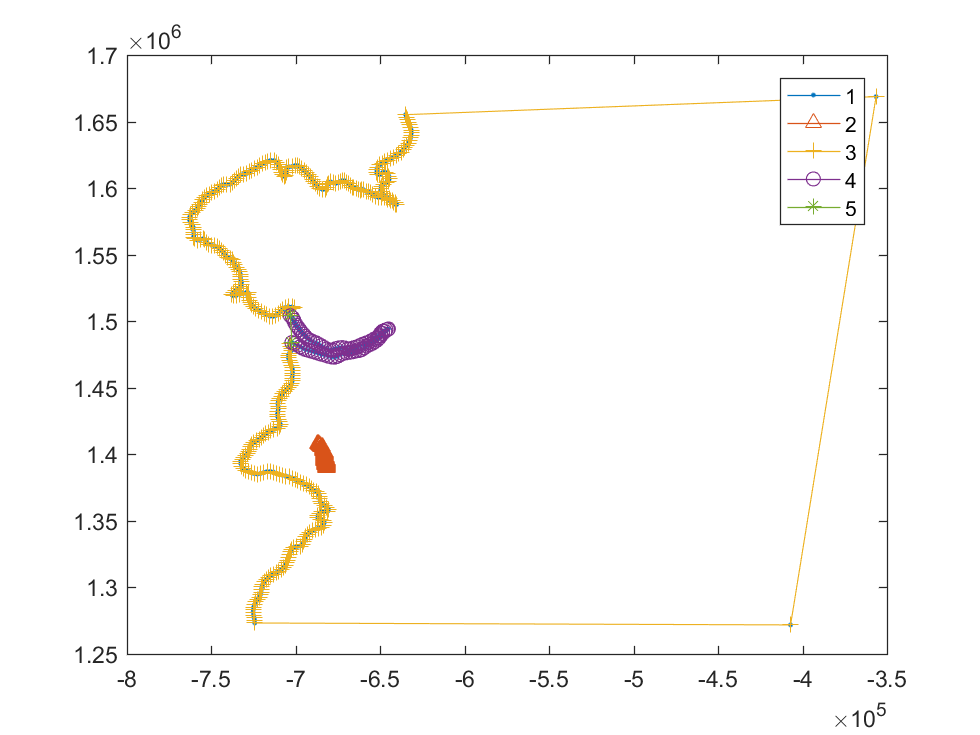
\includegraphics [width=4in]{ExamplesOfMeshGeneration_17.eps}

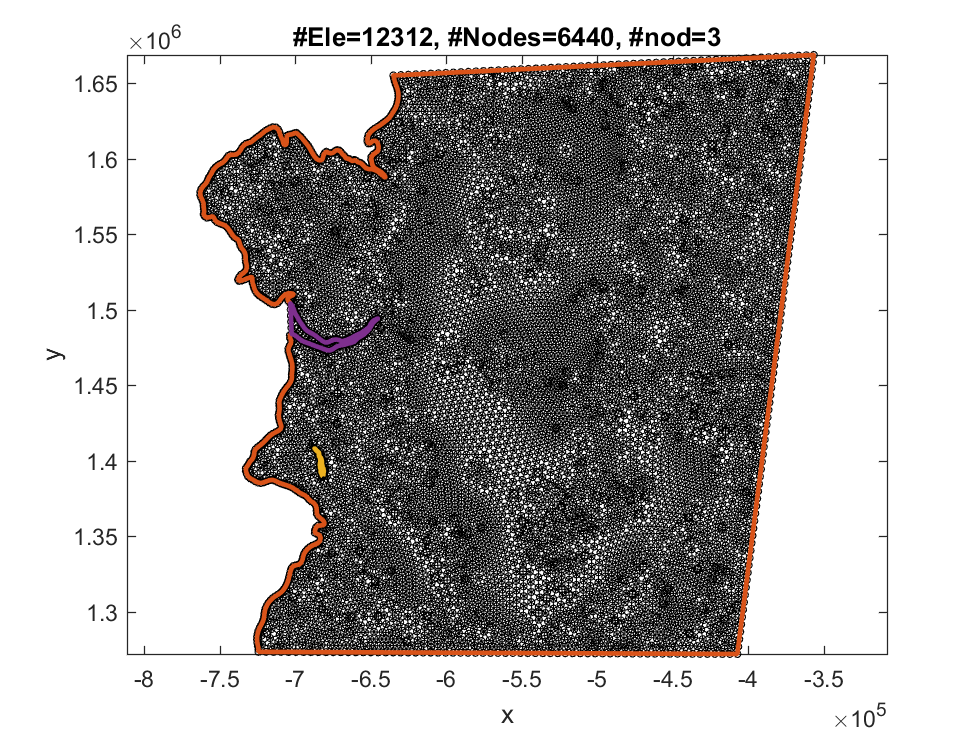
\includegraphics [width=4in]{ExamplesOfMeshGeneration_18.eps}
\begin{par}
example of running gmsh directly for a given input file
\end{par} \vspace{1em}
\begin{verbatim}
status=system([getenv('GmeshHomeDirectory'),'\gmsh.exe GmeshFile.geo -2 -v 5']);
Gmesh=load_gmshGHG('GmeshFile.msh'); % the .msh is a gmsh output file. This file must have be generated previously
TRI=Gmesh.TRIANGLES(1:Gmesh.nbTriangles,1:3);
xy=Gmesh.POS(1:Gmesh.nbNod,1:2);
figure
triplot(TRI,xy(:,1),xy(:,2)) ; axis equal
drawnow
%hold on
%plot(MeshBoundaryCoordinates(:,1),MeshBoundaryCoordinates(:,2),'-or','LineWidth',2)
\end{verbatim}

        \color{lightgray} \begin{verbatim}Info    : Running 'C:\cygwin64\home\Hilmar\ghg\Ua\gmsh-2.11.0-Windows\gmsh.exe GmeshFile.geo -2 -v 5' [Gmsh 2.11.0, 1 node, max. 1 thread]
Info    : Started on Sat Apr 09 18:17:26 2016
Info    : Reading 'GmeshFile.geo'...
Info    : Done reading 'GmeshFile.geo'
Info    : Meshing 1D...
Info    : Meshing curve 1 (Line)
Info    : Meshing curve 2 (Line)
Info    : Meshing curve 3 (Line)
Info    : Meshing curve 4 (Line)
Info    : Meshing curve 5 (Line)
Info    : Meshing curve 6 (Line)
Info    : Meshing curve 7 (Line)
Info    : Meshing curve 8 (Line)
Info    : Meshing curve 9 (Line)
Info    : Meshing curve 10 (Line)
Info    : Meshing curve 11 (Line)
Info    : Meshing curve 12 (Line)
Info    : Meshing curve 13 (Line)
Info    : Meshing curve 14 (Line)
Info    : Meshing curve 15 (Line)
Info    : Meshing curve 16 (Line)
Info    : Meshing curve 17 (Line)
Info    : Meshing curve 18 (Line)
Info    : Meshing curve 19 (Line)
Info    : Meshing curve 20 (Line)
Info    : Meshing curve 21 (Line)
Info    : Meshing curve 22 (Line)
Info    : Meshing curve 23 (Line)
Info    : Meshing curve 24 (Line)
Info    : Meshing curve 25 (Line)
Info    : Meshing curve 26 (Line)
Info    : Meshing curve 27 (Line)
Info    : Meshing curve 28 (Line)
Info    : Meshing curve 29 (Line)
Info    : Meshing curve 30 (Line)
Info    : Meshing curve 31 (Line)
Info    : Meshing curve 32 (Line)
Info    : Meshing curve 33 (Line)
Info    : Meshing curve 34 (Line)
Info    : Meshing curve 35 (Line)
Info    : Meshing curve 36 (Line)
Info    : Meshing curve 37 (Line)
Info    : Meshing curve 38 (Line)
Info    : Meshing curve 39 (Line)
Info    : Meshing curve 40 (Line)
Info    : Meshing curve 41 (Line)
Info    : Meshing curve 42 (Line)
Info    : Meshing curve 43 (Line)
Info    : Meshing curve 44 (Line)
Info    : Meshing curve 45 (Line)
Info    : Meshing curve 46 (Line)
Info    : Meshing curve 47 (Line)
Info    : Meshing curve 48 (Line)
Info    : Meshing curve 49 (Line)
Info    : Meshing curve 50 (Line)
Info    : Meshing curve 51 (Line)
Info    : Meshing curve 52 (Line)
Info    : Meshing curve 53 (Line)
Info    : Meshing curve 54 (Line)
Info    : Meshing curve 55 (Line)
Info    : Meshing curve 56 (Line)
Info    : Meshing curve 57 (Line)
Info    : Meshing curve 58 (Line)
Info    : Meshing curve 59 (Line)
Info    : Meshing curve 60 (Line)
Info    : Meshing curve 61 (Line)
Info    : Meshing curve 62 (Line)
Info    : Meshing curve 63 (Line)
Info    : Meshing curve 64 (Line)
Info    : Meshing curve 65 (Line)
Info    : Meshing curve 66 (Line)
Info    : Meshing curve 67 (Line)
Info    : Meshing curve 68 (Line)
Info    : Meshing curve 69 (Line)
Info    : Meshing curve 70 (Line)
Info    : Meshing curve 71 (Line)
Info    : Meshing curve 72 (Line)
Info    : Meshing curve 73 (Line)
Info    : Meshing curve 74 (Line)
Info    : Meshing curve 75 (Line)
Info    : Meshing curve 76 (Line)
Info    : Meshing curve 77 (Line)
Info    : Meshing curve 78 (Line)
Info    : Meshing curve 79 (Line)
Info    : Meshing curve 80 (Line)
Info    : Meshing curve 81 (Line)
Info    : Meshing curve 82 (Line)
Info    : Meshing curve 83 (Line)
Info    : Meshing curve 84 (Line)
Info    : Meshing curve 85 (Line)
Info    : Meshing curve 86 (Line)
Info    : Meshing curve 87 (Line)
Info    : Meshing curve 88 (Line)
Info    : Meshing curve 89 (Line)
Info    : Meshing curve 90 (Line)
Info    : Meshing curve 91 (Line)
Info    : Meshing curve 92 (Line)
Info    : Meshing curve 93 (Line)
Info    : Meshing curve 94 (Line)
Info    : Meshing curve 95 (Line)
Info    : Meshing curve 96 (Line)
Info    : Meshing curve 97 (Line)
Info    : Meshing curve 98 (Line)
Info    : Meshing curve 99 (Line)
Info    : Meshing curve 100 (Line)
Info    : Meshing curve 101 (Line)
Info    : Meshing curve 102 (Line)
Info    : Meshing curve 103 (Line)
Info    : Meshing curve 104 (Line)
Info    : Meshing curve 105 (Line)
Info    : Meshing curve 106 (Line)
Info    : Meshing curve 107 (Line)
Info    : Meshing curve 108 (Line)
Info    : Meshing curve 109 (Line)
Info    : Meshing curve 110 (Line)
Info    : Meshing curve 111 (Line)
Info    : Meshing curve 112 (Line)
Info    : Meshing curve 113 (Line)
Info    : Meshing curve 114 (Line)
Info    : Meshing curve 115 (Line)
Info    : Meshing curve 116 (Line)
Info    : Meshing curve 117 (Line)
Info    : Meshing curve 118 (Line)
Info    : Meshing curve 119 (Line)
Info    : Meshing curve 120 (Line)
Info    : Meshing curve 121 (Line)
Info    : Meshing curve 122 (Line)
Info    : Meshing curve 123 (Line)
Info    : Meshing curve 124 (Line)
Info    : Meshing curve 125 (Line)
Info    : Meshing curve 126 (Line)
Info    : Meshing curve 127 (Line)
Info    : Meshing curve 128 (Line)
Info    : Meshing curve 129 (Line)
Info    : Meshing curve 130 (Line)
Info    : Meshing curve 131 (Line)
Info    : Meshing curve 132 (Line)
Info    : Meshing curve 133 (Line)
Info    : Meshing curve 134 (Line)
Info    : Meshing curve 135 (Line)
Info    : Meshing curve 136 (Line)
Info    : Meshing curve 137 (Line)
Info    : Meshing curve 138 (Line)
Info    : Meshing curve 139 (Line)
Info    : Meshing curve 140 (Line)
Info    : Meshing curve 141 (Line)
Info    : Meshing curve 142 (Line)
Info    : Meshing curve 143 (Line)
Info    : Meshing curve 144 (Line)
Info    : Meshing curve 145 (Line)
Info    : Meshing curve 146 (Line)
Info    : Meshing curve 147 (Line)
Info    : Meshing curve 148 (Line)
Info    : Meshing curve 149 (Line)
Info    : Meshing curve 150 (Line)
Info    : Meshing curve 151 (Line)
Info    : Meshing curve 152 (Line)
Info    : Meshing curve 153 (Line)
Info    : Meshing curve 154 (Line)
Info    : Meshing curve 155 (Line)
Info    : Meshing curve 156 (Line)
Info    : Meshing curve 157 (Line)
Info    : Meshing curve 158 (Line)
Info    : Meshing curve 159 (Line)
Info    : Meshing curve 160 (Line)
Info    : Meshing curve 161 (Line)
Info    : Meshing curve 162 (Line)
Info    : Meshing curve 163 (Line)
Info    : Meshing curve 164 (Line)
Info    : Meshing curve 165 (Line)
Info    : Meshing curve 166 (Line)
Info    : Meshing curve 167 (Line)
Info    : Meshing curve 168 (Line)
Info    : Meshing curve 169 (Line)
Info    : Meshing curve 170 (Line)
Info    : Meshing curve 171 (Line)
Info    : Meshing curve 172 (Line)
Info    : Meshing curve 173 (Line)
Info    : Meshing curve 174 (Line)
Info    : Meshing curve 175 (Line)
Info    : Meshing curve 176 (Line)
Info    : Meshing curve 177 (Line)
Info    : Meshing curve 178 (Line)
Info    : Meshing curve 179 (Line)
Info    : Meshing curve 180 (Line)
Info    : Meshing curve 181 (Line)
Info    : Meshing curve 182 (Line)
Info    : Meshing curve 183 (Line)
Info    : Meshing curve 184 (Line)
Info    : Meshing curve 185 (Line)
Info    : Meshing curve 186 (Line)
Info    : Meshing curve 187 (Line)
Info    : Meshing curve 188 (Line)
Info    : Meshing curve 189 (Line)
Info    : Meshing curve 190 (Line)
Info    : Meshing curve 191 (Line)
Info    : Meshing curve 192 (Line)
Info    : Meshing curve 193 (Line)
Info    : Meshing curve 194 (Line)
Info    : Meshing curve 195 (Line)
Info    : Meshing curve 196 (Line)
Info    : Meshing curve 197 (Line)
Info    : Meshing curve 198 (Line)
Info    : Meshing curve 199 (Line)
Info    : Meshing curve 200 (Line)
Info    : Meshing curve 201 (Line)
Info    : Meshing curve 202 (Line)
Info    : Meshing curve 203 (Line)
Info    : Meshing curve 204 (Line)
Info    : Meshing curve 205 (Line)
Info    : Meshing curve 206 (Line)
Info    : Meshing curve 207 (Line)
Info    : Meshing curve 208 (Line)
Info    : Meshing curve 209 (Line)
Info    : Meshing curve 210 (Line)
Info    : Meshing curve 211 (Line)
Info    : Meshing curve 212 (Line)
Info    : Meshing curve 213 (Line)
Info    : Meshing curve 214 (Line)
Info    : Meshing curve 215 (Line)
Info    : Meshing curve 216 (Line)
Info    : Meshing curve 217 (Line)
Info    : Meshing curve 218 (Line)
Info    : Meshing curve 219 (Line)
Info    : Meshing curve 220 (Line)
Info    : Meshing curve 221 (Line)
Info    : Meshing curve 222 (Line)
Info    : Meshing curve 223 (Line)
Info    : Meshing curve 224 (Line)
Info    : Meshing curve 225 (Line)
Info    : Meshing curve 226 (Line)
Info    : Meshing curve 227 (Line)
Info    : Meshing curve 228 (Line)
Info    : Meshing curve 229 (Line)
Info    : Meshing curve 230 (Line)
Info    : Meshing curve 231 (Line)
Info    : Meshing curve 232 (Line)
Info    : Meshing curve 233 (Line)
Info    : Meshing curve 234 (Line)
Info    : Meshing curve 235 (Line)
Info    : Meshing curve 236 (Line)
Info    : Meshing curve 237 (Line)
Info    : Meshing curve 238 (Line)
Info    : Meshing curve 239 (Line)
Info    : Meshing curve 240 (Line)
Info    : Meshing curve 241 (Line)
Info    : Meshing curve 242 (Line)
Info    : Meshing curve 243 (Line)
Info    : Meshing curve 244 (Line)
Info    : Meshing curve 245 (Line)
Info    : Meshing curve 246 (Line)
Info    : Meshing curve 247 (Line)
Info    : Meshing curve 248 (Line)
Info    : Meshing curve 249 (Line)
Info    : Meshing curve 250 (Line)
Info    : Meshing curve 251 (Line)
Info    : Meshing curve 252 (Line)
Info    : Meshing curve 253 (Line)
Info    : Meshing curve 254 (Line)
Info    : Meshing curve 255 (Line)
Info    : Meshing curve 256 (Line)
Info    : Meshing curve 257 (Line)
Info    : Meshing curve 258 (Line)
Info    : Meshing curve 259 (Line)
Info    : Meshing curve 260 (Line)
Info    : Meshing curve 261 (Line)
Info    : Meshing curve 262 (Line)
Info    : Meshing curve 263 (Line)
Info    : Meshing curve 264 (Line)
Info    : Meshing curve 265 (Line)
Info    : Meshing curve 266 (Line)
Info    : Meshing curve 267 (Line)
Info    : Meshing curve 268 (Line)
Info    : Meshing curve 269 (Line)
Info    : Meshing curve 270 (Line)
Info    : Meshing curve 271 (Line)
Info    : Meshing curve 272 (Line)
Info    : Meshing curve 273 (Line)
Info    : Meshing curve 274 (Line)
Info    : Meshing curve 275 (Line)
Info    : Meshing curve 276 (Line)
Info    : Meshing curve 277 (Line)
Info    : Meshing curve 278 (Line)
Info    : Meshing curve 279 (Line)
Info    : Meshing curve 280 (Line)
Info    : Meshing curve 281 (Line)
Info    : Meshing curve 282 (Line)
Info    : Meshing curve 283 (Line)
Info    : Meshing curve 284 (Line)
Info    : Meshing curve 285 (Line)
Info    : Meshing curve 286 (Line)
Info    : Meshing curve 287 (Line)
Info    : Meshing curve 288 (Line)
Info    : Meshing curve 289 (Line)
Info    : Meshing curve 290 (Line)
Info    : Meshing curve 291 (Line)
Info    : Meshing curve 292 (Line)
Info    : Meshing curve 293 (Line)
Info    : Meshing curve 294 (Line)
Info    : Meshing curve 295 (Line)
Info    : Meshing curve 296 (Line)
Info    : Meshing curve 297 (Line)
Info    : Meshing curve 298 (Line)
Info    : Meshing curve 299 (Line)
Info    : Meshing curve 300 (Line)
Info    : Meshing curve 301 (Line)
Info    : Meshing curve 302 (Line)
Info    : Meshing curve 303 (Line)
Info    : Meshing curve 304 (Line)
Info    : Meshing curve 305 (Line)
Info    : Meshing curve 306 (Line)
Info    : Meshing curve 307 (Line)
Info    : Meshing curve 308 (Line)
Info    : Meshing curve 309 (Line)
Info    : Meshing curve 310 (Line)
Info    : Meshing curve 311 (Line)
Info    : Meshing curve 312 (Line)
Info    : Meshing curve 313 (Line)
Info    : Meshing curve 314 (Line)
Info    : Meshing curve 315 (Line)
Info    : Meshing curve 316 (Line)
Info    : Meshing curve 317 (Line)
Info    : Meshing curve 318 (Line)
Info    : Meshing curve 319 (Line)
Info    : Meshing curve 320 (Line)
Info    : Meshing curve 321 (Line)
Info    : Meshing curve 322 (Line)
Info    : Meshing curve 323 (Line)
Info    : Meshing curve 324 (Line)
Info    : Meshing curve 325 (Line)
Info    : Meshing curve 326 (Line)
Info    : Meshing curve 327 (Line)
Info    : Meshing curve 328 (Line)
Info    : Meshing curve 329 (Line)
Info    : Meshing curve 330 (Line)
Info    : Meshing curve 331 (Line)
Info    : Meshing curve 332 (Line)
Info    : Meshing curve 333 (Line)
Info    : Meshing curve 334 (Line)
Info    : Meshing curve 335 (Line)
Info    : Meshing curve 336 (Line)
Info    : Meshing curve 337 (Line)
Info    : Meshing curve 338 (Line)
Info    : Meshing curve 339 (Line)
Info    : Meshing curve 340 (Line)
Info    : Meshing curve 341 (Line)
Info    : Meshing curve 342 (Line)
Info    : Meshing curve 343 (Line)
Info    : Meshing curve 344 (Line)
Info    : Meshing curve 345 (Line)
Info    : Meshing curve 346 (Line)
Info    : Meshing curve 347 (Line)
Info    : Meshing curve 348 (Line)
Info    : Meshing curve 349 (Line)
Info    : Meshing curve 350 (Line)
Info    : Meshing curve 351 (Line)
Info    : Meshing curve 352 (Line)
Info    : Meshing curve 353 (Line)
Info    : Meshing curve 354 (Line)
Info    : Meshing curve 355 (Line)
Info    : Meshing curve 356 (Line)
Info    : Meshing curve 357 (Line)
Info    : Meshing curve 358 (Line)
Info    : Meshing curve 359 (Line)
Info    : Meshing curve 360 (Line)
Info    : Meshing curve 361 (Line)
Info    : Meshing curve 362 (Line)
Info    : Meshing curve 363 (Line)
Info    : Meshing curve 364 (Line)
Info    : Meshing curve 365 (Line)
Info    : Meshing curve 366 (Line)
Info    : Meshing curve 367 (Line)
Info    : Meshing curve 368 (Line)
Info    : Meshing curve 369 (Line)
Info    : Meshing curve 370 (Line)
Info    : Meshing curve 371 (Line)
Info    : Meshing curve 372 (Line)
Info    : Meshing curve 373 (Line)
Info    : Meshing curve 374 (Line)
Info    : Meshing curve 375 (Line)
Info    : Meshing curve 376 (Line)
Info    : Meshing curve 377 (Line)
Info    : Meshing curve 378 (Line)
Info    : Meshing curve 379 (Line)
Info    : Meshing curve 380 (Line)
Info    : Meshing curve 381 (Line)
Info    : Meshing curve 382 (Line)
Info    : Meshing curve 383 (Line)
Info    : Meshing curve 384 (Line)
Info    : Meshing curve 385 (Line)
Info    : Meshing curve 386 (Line)
Info    : Meshing curve 387 (Line)
Info    : Meshing curve 388 (Line)
Info    : Meshing curve 389 (Line)
Info    : Meshing curve 390 (Line)
Info    : Meshing curve 391 (Line)
Info    : Meshing curve 392 (Line)
Info    : Meshing curve 393 (Line)
Info    : Meshing curve 394 (Line)
Info    : Meshing curve 395 (Line)
Info    : Meshing curve 396 (Line)
Info    : Meshing curve 397 (Line)
Info    : Meshing curve 398 (Line)
Info    : Meshing curve 399 (Line)
Info    : Meshing curve 400 (Line)
Info    : Meshing curve 401 (Line)
Info    : Meshing curve 402 (Line)
Info    : Meshing curve 403 (Line)
Info    : Meshing curve 404 (Line)
Info    : Meshing curve 405 (Line)
Info    : Meshing curve 406 (Line)
Info    : Meshing curve 407 (Line)
Info    : Meshing curve 408 (Line)
Info    : Meshing curve 409 (Line)
Info    : Meshing curve 410 (Line)
Info    : Meshing curve 411 (Line)
Info    : Meshing curve 412 (Line)
Info    : Meshing curve 413 (Line)
Info    : Meshing curve 414 (Line)
Info    : Meshing curve 415 (Line)
Info    : Meshing curve 416 (Line)
Info    : Meshing curve 417 (Line)
Info    : Meshing curve 418 (Line)
Info    : Meshing curve 419 (Line)
Info    : Meshing curve 420 (Line)
Info    : Meshing curve 421 (Line)
Info    : Meshing curve 422 (Line)
Info    : Meshing curve 423 (Line)
Info    : Meshing curve 424 (Line)
Info    : Meshing curve 425 (Line)
Info    : Meshing curve 426 (Line)
Info    : Meshing curve 427 (Line)
Info    : Meshing curve 428 (Line)
Info    : Meshing curve 429 (Line)
Info    : Meshing curve 430 (Line)
Info    : Meshing curve 431 (Line)
Info    : Meshing curve 432 (Line)
Info    : Meshing curve 433 (Line)
Info    : Meshing curve 434 (Line)
Info    : Meshing curve 435 (Line)
Info    : Meshing curve 436 (Line)
Info    : Meshing curve 437 (Line)
Info    : Meshing curve 438 (Line)
Info    : Meshing curve 439 (Line)
Info    : Meshing curve 440 (Line)
Info    : Meshing curve 441 (Line)
Info    : Meshing curve 442 (Line)
Info    : Meshing curve 443 (Line)
Info    : Meshing curve 444 (Line)
Info    : Meshing curve 445 (Line)
Info    : Meshing curve 446 (Line)
Info    : Meshing curve 447 (Line)
Info    : Meshing curve 448 (Line)
Info    : Meshing curve 449 (Line)
Info    : Meshing curve 450 (Line)
Info    : Meshing curve 451 (Line)
Info    : Meshing curve 452 (Line)
Info    : Meshing curve 453 (Line)
Info    : Meshing curve 454 (Line)
Info    : Meshing curve 455 (Line)
Info    : Meshing curve 456 (Line)
Info    : Meshing curve 457 (Line)
Info    : Meshing curve 458 (Line)
Info    : Meshing curve 459 (Line)
Info    : Meshing curve 460 (Line)
Info    : Meshing curve 461 (Line)
Info    : Meshing curve 462 (Line)
Info    : Meshing curve 463 (Line)
Info    : Meshing curve 464 (Line)
Info    : Meshing curve 465 (Line)
Info    : Meshing curve 466 (Line)
Info    : Meshing curve 467 (Line)
Info    : Meshing curve 468 (Line)
Info    : Meshing curve 469 (Line)
Info    : Meshing curve 470 (Line)
Info    : Meshing curve 471 (Line)
Info    : Meshing curve 472 (Line)
Info    : Meshing curve 473 (Line)
Info    : Meshing curve 474 (Line)
Info    : Meshing curve 475 (Line)
Info    : Meshing curve 476 (Line)
Info    : Meshing curve 477 (Line)
Info    : Meshing curve 478 (Line)
Info    : Meshing curve 479 (Line)
Info    : Meshing curve 480 (Line)
Info    : Meshing curve 481 (Line)
Info    : Meshing curve 482 (Line)
Info    : Meshing curve 483 (Line)
Info    : Meshing curve 484 (Line)
Info    : Meshing curve 485 (Line)
Info    : Meshing curve 486 (Line)
Info    : Meshing curve 487 (Line)
Info    : Meshing curve 488 (Line)
Info    : Meshing curve 489 (Line)
Info    : Meshing curve 490 (Line)
Info    : Meshing curve 491 (Line)
Info    : Meshing curve 492 (Line)
Info    : Meshing curve 493 (Line)
Info    : Meshing curve 494 (Line)
Info    : Meshing curve 495 (Line)
Info    : Meshing curve 496 (Line)
Info    : Meshing curve 497 (Line)
Info    : Meshing curve 498 (Line)
Info    : Meshing curve 499 (Line)
Info    : Meshing curve 500 (Line)
Info    : Meshing curve 501 (Line)
Info    : Meshing curve 502 (Line)
Info    : Meshing curve 503 (Line)
Info    : Meshing curve 504 (Line)
Info    : Meshing curve 505 (Line)
Info    : Meshing curve 506 (Line)
Info    : Meshing curve 507 (Line)
Info    : Meshing curve 508 (Line)
Info    : Meshing curve 509 (Line)
Info    : Meshing curve 510 (Line)
Info    : Meshing curve 511 (Line)
Info    : Meshing curve 512 (Line)
Info    : Meshing curve 513 (Line)
Info    : Meshing curve 514 (Line)
Info    : Meshing curve 515 (Line)
Info    : Meshing curve 516 (Line)
Info    : Meshing curve 517 (Line)
Info    : Meshing curve 518 (Line)
Info    : Meshing curve 519 (Line)
Info    : Meshing curve 520 (Line)
Info    : Meshing curve 521 (Line)
Info    : Meshing curve 522 (Line)
Info    : Meshing curve 523 (Line)
Info    : Meshing curve 524 (Line)
Info    : Meshing curve 525 (Line)
Info    : Meshing curve 526 (Line)
Info    : Meshing curve 527 (Line)
Info    : Meshing curve 528 (Line)
Info    : Meshing curve 529 (Line)
Info    : Meshing curve 530 (Line)
Info    : Meshing curve 531 (Line)
Info    : Meshing curve 532 (Line)
Info    : Meshing curve 533 (Line)
Info    : Meshing curve 534 (Line)
Info    : Meshing curve 535 (Line)
Info    : Meshing curve 536 (Line)
Info    : Meshing curve 537 (Line)
Info    : Meshing curve 538 (Line)
Info    : Meshing curve 539 (Line)
Info    : Meshing curve 540 (Line)
Info    : Meshing curve 541 (Line)
Info    : Meshing curve 542 (Line)
Info    : Meshing curve 543 (Line)
Info    : Meshing curve 544 (Line)
Info    : Meshing curve 545 (Line)
Info    : Meshing curve 546 (Line)
Info    : Meshing curve 547 (Line)
Info    : Meshing curve 548 (Line)
Info    : Meshing curve 549 (Line)
Info    : Meshing curve 550 (Line)
Info    : Meshing curve 551 (Line)
Info    : Meshing curve 552 (Line)
Info    : Meshing curve 553 (Line)
Info    : Meshing curve 554 (Line)
Info    : Meshing curve 555 (Line)
Info    : Meshing curve 556 (Line)
Info    : Meshing curve 557 (Line)
Info    : Meshing curve 558 (Line)
Info    : Meshing curve 559 (Line)
Info    : Meshing curve 560 (Line)
Info    : Meshing curve 561 (Line)
Info    : Meshing curve 562 (Line)
Info    : Meshing curve 563 (Line)
Info    : Meshing curve 564 (Line)
Info    : Meshing curve 565 (Line)
Info    : Meshing curve 566 (Line)
Info    : Meshing curve 567 (Line)
Info    : Meshing curve 568 (Line)
Info    : Meshing curve 569 (Line)
Info    : Meshing curve 570 (Line)
Info    : Meshing curve 571 (Line)
Info    : Meshing curve 572 (Line)
Info    : Meshing curve 573 (Line)
Info    : Meshing curve 574 (Line)
Info    : Meshing curve 575 (Line)
Info    : Meshing curve 576 (Line)
Info    : Meshing curve 577 (Line)
Info    : Meshing curve 578 (Line)
Info    : Meshing curve 579 (Line)
Info    : Meshing curve 580 (Line)
Info    : Meshing curve 581 (Line)
Info    : Meshing curve 582 (Line)
Info    : Meshing curve 583 (Line)
Info    : Meshing curve 584 (Line)
Info    : Meshing curve 585 (Line)
Info    : Meshing curve 586 (Line)
Info    : Meshing curve 587 (Line)
Info    : Meshing curve 588 (Line)
Info    : Meshing curve 589 (Line)
Info    : Meshing curve 590 (Line)
Info    : Meshing curve 591 (Line)
Info    : Meshing curve 592 (Line)
Info    : Meshing curve 593 (Line)
Info    : Meshing curve 594 (Line)
Info    : Meshing curve 595 (Line)
Info    : Meshing curve 596 (Line)
Info    : Meshing curve 597 (Line)
Info    : Meshing curve 598 (Line)
Info    : Meshing curve 599 (Line)
Info    : Meshing curve 600 (Line)
Info    : Meshing curve 601 (Line)
Info    : Meshing curve 602 (Line)
Info    : Meshing curve 603 (Line)
Info    : Meshing curve 604 (Line)
Info    : Meshing curve 605 (Line)
Info    : Meshing curve 606 (Line)
Info    : Meshing curve 607 (Line)
Info    : Meshing curve 608 (Line)
Info    : Meshing curve 609 (Line)
Info    : Meshing curve 610 (Line)
Info    : Meshing curve 611 (Line)
Info    : Meshing curve 612 (Line)
Info    : Meshing curve 613 (Line)
Info    : Meshing curve 614 (Line)
Info    : Meshing curve 615 (Line)
Info    : Meshing curve 616 (Line)
Info    : Meshing curve 617 (Line)
Info    : Meshing curve 618 (Line)
Info    : Meshing curve 619 (Line)
Info    : Meshing curve 620 (Line)
Info    : Meshing curve 621 (Line)
Info    : Meshing curve 622 (Line)
Info    : Meshing curve 623 (Line)
Info    : Meshing curve 624 (Line)
Info    : Meshing curve 625 (Line)
Info    : Meshing curve 626 (Line)
Info    : Meshing curve 627 (Line)
Info    : Meshing curve 628 (Line)
Info    : Meshing curve 629 (Line)
Info    : Meshing curve 630 (Line)
Info    : Meshing curve 631 (Line)
Info    : Meshing curve 632 (Line)
Info    : Meshing curve 633 (Line)
Info    : Meshing curve 634 (Line)
Info    : Meshing curve 635 (Line)
Info    : Meshing curve 636 (Line)
Info    : Meshing curve 637 (Line)
Info    : Meshing curve 638 (Line)
Info    : Meshing curve 639 (Line)
Info    : Meshing curve 640 (Line)
Info    : Meshing curve 641 (Line)
Info    : Meshing curve 642 (Line)
Info    : Meshing curve 643 (Line)
Info    : Meshing curve 644 (Line)
Info    : Meshing curve 645 (Line)
Info    : Meshing curve 646 (Line)
Info    : Meshing curve 647 (Line)
Info    : Meshing curve 648 (Line)
Info    : Meshing curve 649 (Line)
Info    : Meshing curve 650 (Line)
Info    : Meshing curve 651 (Line)
Info    : Meshing curve 652 (Line)
Info    : Meshing curve 653 (Line)
Info    : Meshing curve 654 (Line)
Info    : Meshing curve 655 (Line)
Info    : Meshing curve 656 (Line)
Info    : Meshing curve 657 (Line)
Info    : Meshing curve 658 (Line)
Info    : Meshing curve 659 (Line)
Info    : Meshing curve 660 (Line)
Info    : Meshing curve 661 (Line)
Info    : Meshing curve 662 (Line)
Info    : Meshing curve 663 (Line)
Info    : Meshing curve 664 (Line)
Info    : Meshing curve 665 (Line)
Info    : Meshing curve 666 (Line)
Info    : Meshing curve 667 (Line)
Info    : Meshing curve 668 (Line)
Info    : Meshing curve 669 (Line)
Info    : Meshing curve 670 (Line)
Info    : Meshing curve 671 (Line)
Info    : Meshing curve 672 (Line)
Info    : Meshing curve 673 (Line)
Info    : Meshing curve 674 (Line)
Info    : Meshing curve 675 (Line)
Info    : Meshing curve 676 (Line)
Info    : Meshing curve 677 (Line)
Info    : Meshing curve 678 (Line)
Info    : Meshing curve 679 (Line)
Info    : Meshing curve 680 (Line)
Info    : Meshing curve 681 (Line)
Info    : Meshing curve 682 (Line)
Info    : Meshing curve 683 (Line)
Info    : Meshing curve 684 (Line)
Info    : Meshing curve 685 (Line)
Info    : Meshing curve 686 (Line)
Info    : Meshing curve 687 (Line)
Info    : Meshing curve 688 (Line)
Info    : Meshing curve 689 (Line)
Info    : Meshing curve 690 (Line)
Info    : Meshing curve 691 (Line)
Info    : Meshing curve 692 (Line)
Info    : Meshing curve 693 (Line)
Info    : Meshing curve 694 (Line)
Info    : Meshing curve 695 (Line)
Info    : Meshing curve 696 (Line)
Info    : Meshing curve 697 (Line)
Info    : Meshing curve 698 (Line)
Info    : Meshing curve 699 (Line)
Info    : Meshing curve 700 (Line)
Info    : Meshing curve 701 (Line)
Info    : Meshing curve 702 (Line)
Info    : Meshing curve 703 (Line)
Info    : Meshing curve 704 (Line)
Info    : Meshing curve 705 (Line)
Info    : Meshing curve 706 (Line)
Info    : Meshing curve 707 (Line)
Info    : Meshing curve 708 (Line)
Info    : Meshing curve 709 (Line)
Info    : Meshing curve 710 (Line)
Info    : Meshing curve 711 (Line)
Info    : Meshing curve 712 (Line)
Info    : Meshing curve 713 (Line)
Info    : Meshing curve 714 (Line)
Info    : Meshing curve 715 (Line)
Info    : Meshing curve 716 (Line)
Info    : Meshing curve 717 (Line)
Info    : Meshing curve 718 (Line)
Info    : Meshing curve 719 (Line)
Info    : Meshing curve 720 (Line)
Info    : Meshing curve 721 (Line)
Info    : Meshing curve 722 (Line)
Info    : Meshing curve 723 (Line)
Info    : Meshing curve 724 (Line)
Info    : Meshing curve 725 (Line)
Info    : Meshing curve 726 (Line)
Info    : Meshing curve 727 (Line)
Info    : Meshing curve 728 (Line)
Info    : Meshing curve 729 (Line)
Info    : Meshing curve 730 (Line)
Info    : Meshing curve 731 (Line)
Info    : Meshing curve 732 (Line)
Info    : Meshing curve 733 (Line)
Info    : Meshing curve 734 (Line)
Info    : Meshing curve 735 (Line)
Info    : Meshing curve 736 (Line)
Info    : Meshing curve 737 (Line)
Info    : Meshing curve 738 (Line)
Info    : Meshing curve 739 (Line)
Info    : Meshing curve 740 (Line)
Info    : Meshing curve 741 (Line)
Info    : Meshing curve 742 (Line)
Info    : Meshing curve 743 (Line)
Info    : Meshing curve 744 (Line)
Info    : Meshing curve 745 (Line)
Info    : Meshing curve 746 (Line)
Info    : Meshing curve 747 (Line)
Info    : Meshing curve 748 (Line)
Info    : Meshing curve 749 (Line)
Info    : Meshing curve 750 (Line)
Info    : Meshing curve 751 (Line)
Info    : Meshing curve 752 (Line)
Info    : Meshing curve 753 (Line)
Info    : Meshing curve 754 (Line)
Info    : Meshing curve 755 (Line)
Info    : Meshing curve 756 (Line)
Info    : Meshing curve 757 (Line)
Info    : Meshing curve 758 (Line)
Info    : Meshing curve 759 (Line)
Info    : Meshing curve 760 (Line)
Info    : Meshing curve 761 (Line)
Info    : Meshing curve 762 (Line)
Info    : Meshing curve 763 (Line)
Info    : Meshing curve 764 (Line)
Info    : Meshing curve 765 (Line)
Info    : Meshing curve 766 (Line)
Info    : Meshing curve 767 (Line)
Info    : Meshing curve 768 (Line)
Info    : Meshing curve 769 (Line)
Info    : Meshing curve 770 (Line)
Info    : Meshing curve 771 (Line)
Info    : Meshing curve 772 (Line)
Info    : Meshing curve 773 (Line)
Info    : Meshing curve 774 (Line)
Info    : Meshing curve 775 (Line)
Info    : Meshing curve 776 (Line)
Info    : Meshing curve 777 (Line)
Info    : Meshing curve 778 (Line)
Info    : Meshing curve 779 (Line)
Info    : Meshing curve 780 (Line)
Info    : Meshing curve 781 (Line)
Info    : Meshing curve 782 (Line)
Info    : Meshing curve 783 (Line)
Info    : Meshing curve 784 (Line)
Info    : Meshing curve 785 (Line)
Info    : Meshing curve 786 (Line)
Info    : Meshing curve 787 (Line)
Info    : Meshing curve 788 (Line)
Info    : Meshing curve 789 (Line)
Info    : Meshing curve 790 (Line)
Info    : Meshing curve 791 (Line)
Info    : Meshing curve 792 (Line)
Info    : Meshing curve 793 (Line)
Info    : Meshing curve 794 (Line)
Info    : Meshing curve 795 (Line)
Info    : Meshing curve 796 (Line)
Info    : Meshing curve 797 (Line)
Info    : Meshing curve 798 (Line)
Info    : Meshing curve 799 (Line)
Info    : Meshing curve 800 (Line)
Info    : Meshing curve 801 (Line)
Info    : Meshing curve 802 (Line)
Info    : Meshing curve 803 (Line)
Info    : Meshing curve 804 (Line)
Info    : Meshing curve 805 (Line)
Info    : Meshing curve 806 (Line)
Info    : Meshing curve 807 (Line)
Info    : Meshing curve 808 (Line)
Info    : Meshing curve 809 (Line)
Info    : Meshing curve 810 (Line)
Info    : Meshing curve 811 (Line)
Info    : Meshing curve 812 (Line)
Info    : Meshing curve 813 (Line)
Info    : Meshing curve 814 (Line)
Info    : Meshing curve 815 (Line)
Info    : Meshing curve 816 (Line)
Info    : Meshing curve 817 (Line)
Info    : Meshing curve 818 (Line)
Info    : Meshing curve 819 (Line)
Info    : Meshing curve 820 (Line)
Info    : Meshing curve 821 (Line)
Info    : Meshing curve 822 (Line)
Info    : Meshing curve 823 (Line)
Info    : Meshing curve 824 (Line)
Info    : Meshing curve 825 (Line)
Info    : Meshing curve 826 (Line)
Info    : Meshing curve 827 (Line)
Info    : Meshing curve 828 (Line)
Info    : Meshing curve 829 (Line)
Info    : Meshing curve 830 (Line)
Info    : Meshing curve 831 (Line)
Info    : Meshing curve 832 (Line)
Info    : Meshing curve 833 (Line)
Info    : Meshing curve 834 (Line)
Info    : Meshing curve 835 (Line)
Info    : Meshing curve 836 (Line)
Info    : Meshing curve 837 (Line)
Info    : Meshing curve 838 (Line)
Info    : Meshing curve 839 (Line)
Info    : Meshing curve 840 (Line)
Info    : Meshing curve 841 (Line)
Info    : Meshing curve 842 (Line)
Info    : Meshing curve 843 (Line)
Info    : Meshing curve 844 (Line)
Info    : Meshing curve 845 (Line)
Info    : Meshing curve 846 (Line)
Info    : Meshing curve 847 (Line)
Info    : Meshing curve 848 (Line)
Info    : Meshing curve 849 (Line)
Info    : Meshing curve 850 (Line)
Info    : Meshing curve 851 (Line)
Info    : Meshing curve 852 (Line)
Info    : Meshing curve 853 (Line)
Info    : Meshing curve 854 (Line)
Info    : Meshing curve 855 (Line)
Info    : Meshing curve 856 (Line)
Info    : Meshing curve 857 (Line)
Info    : Meshing curve 858 (Line)
Info    : Meshing curve 859 (Line)
Info    : Meshing curve 860 (Line)
Info    : Meshing curve 861 (Line)
Info    : Meshing curve 862 (Line)
Info    : Meshing curve 863 (Line)
Info    : Meshing curve 864 (Line)
Info    : Meshing curve 865 (Line)
Info    : Meshing curve 866 (Line)
Info    : Meshing curve 867 (Line)
Info    : Meshing curve 868 (Line)
Info    : Meshing curve 869 (Line)
Info    : Meshing curve 870 (Line)
Info    : Meshing curve 871 (Line)
Info    : Meshing curve 872 (Line)
Info    : Meshing curve 873 (Line)
Info    : Meshing curve 874 (Line)
Info    : Meshing curve 875 (Line)
Info    : Meshing curve 876 (Line)
Info    : Meshing curve 877 (Line)
Info    : Meshing curve 878 (Line)
Info    : Meshing curve 879 (Line)
Info    : Meshing curve 880 (Line)
Info    : Meshing curve 881 (Line)
Info    : Meshing curve 882 (Line)
Info    : Meshing curve 883 (Line)
Info    : Meshing curve 884 (Line)
Info    : Meshing curve 885 (Line)
Info    : Meshing curve 886 (Line)
Info    : Meshing curve 887 (Line)
Info    : Meshing curve 888 (Line)
Info    : Meshing curve 889 (Line)
Info    : Meshing curve 890 (Line)
Info    : Meshing curve 891 (Line)
Info    : Meshing curve 892 (Line)
Info    : Meshing curve 893 (Line)
Info    : Meshing curve 894 (Line)
Info    : Meshing curve 895 (Line)
Info    : Meshing curve 896 (Line)
Info    : Meshing curve 897 (Line)
Info    : Meshing curve 898 (Line)
Info    : Meshing curve 899 (Line)
Info    : Meshing curve 900 (Line)
Info    : Meshing curve 901 (Line)
Info    : Meshing curve 902 (Line)
Info    : Meshing curve 903 (Line)
Info    : Meshing curve 904 (Line)
Info    : Meshing curve 905 (Line)
Info    : Meshing curve 906 (Line)
Info    : Meshing curve 907 (Line)
Info    : Meshing curve 908 (Line)
Info    : Meshing curve 909 (Line)
Info    : Meshing curve 910 (Line)
Info    : Meshing curve 911 (Line)
Info    : Meshing curve 912 (Line)
Info    : Meshing curve 913 (Line)
Info    : Meshing curve 914 (Line)
Info    : Meshing curve 915 (Line)
Info    : Meshing curve 916 (Line)
Info    : Meshing curve 917 (Line)
Info    : Meshing curve 918 (Line)
Info    : Meshing curve 919 (Line)
Info    : Meshing curve 920 (Line)
Info    : Meshing curve 921 (Line)
Info    : Meshing curve 922 (Line)
Info    : Meshing curve 923 (Line)
Info    : Meshing curve 924 (Line)
Info    : Meshing curve 925 (Line)
Info    : Meshing curve 926 (Line)
Info    : Meshing curve 927 (Line)
Info    : Meshing curve 928 (Line)
Info    : Meshing curve 929 (Line)
Info    : Meshing curve 930 (Line)
Info    : Meshing curve 931 (Line)
Info    : Meshing curve 932 (Line)
Info    : Meshing curve 933 (Line)
Info    : Meshing curve 934 (Line)
Info    : Meshing curve 935 (Line)
Info    : Meshing curve 936 (Line)
Info    : Meshing curve 937 (Line)
Info    : Meshing curve 938 (Line)
Info    : Meshing curve 939 (Line)
Info    : Meshing curve 940 (Line)
Info    : Meshing curve 941 (Line)
Info    : Meshing curve 942 (Line)
Info    : Meshing curve 943 (Line)
Info    : Meshing curve 944 (Line)
Info    : Meshing curve 945 (Line)
Info    : Meshing curve 946 (Line)
Info    : Meshing curve 947 (Line)
Info    : Meshing curve 948 (Line)
Info    : Meshing curve 949 (Line)
Info    : Meshing curve 950 (Line)
Info    : Meshing curve 951 (Line)
Info    : Meshing curve 952 (Line)
Info    : Meshing curve 953 (Line)
Info    : Meshing curve 954 (Line)
Info    : Meshing curve 955 (Line)
Info    : Meshing curve 956 (Line)
Info    : Meshing curve 957 (Line)
Info    : Meshing curve 958 (Line)
Info    : Meshing curve 959 (Line)
Info    : Meshing curve 960 (Line)
Info    : Meshing curve 961 (Line)
Info    : Meshing curve 962 (Line)
Info    : Meshing curve 963 (Line)
Info    : Meshing curve 964 (Line)
Info    : Meshing curve 965 (Line)
Info    : Meshing curve 966 (Line)
Info    : Meshing curve 967 (Line)
Info    : Meshing curve 968 (Line)
Info    : Meshing curve 969 (Line)
Info    : Meshing curve 970 (Line)
Info    : Meshing curve 971 (Line)
Info    : Meshing curve 972 (Line)
Info    : Meshing curve 973 (Line)
Info    : Meshing curve 974 (Line)
Info    : Meshing curve 975 (Line)
Info    : Meshing curve 976 (Line)
Info    : Meshing curve 977 (Line)
Info    : Meshing curve 978 (Line)
Info    : Meshing curve 979 (Line)
Info    : Meshing curve 980 (Line)
Info    : Meshing curve 981 (Line)
Info    : Meshing curve 982 (Line)
Info    : Meshing curve 983 (Line)
Info    : Meshing curve 984 (Line)
Info    : Meshing curve 985 (Line)
Info    : Meshing curve 986 (Line)
Info    : Meshing curve 987 (Line)
Info    : Meshing curve 988 (Line)
Info    : Meshing curve 989 (Line)
Info    : Meshing curve 990 (Line)
Info    : Meshing curve 991 (Line)
Info    : Meshing curve 992 (Line)
Info    : Done meshing 1D (0.03125 s)
Info    : Meshing 2D...
Info    : Meshing surface 1 (Plane, MeshAdapt)
Info    : Meshing surface 2 (Plane, MeshAdapt)
Info    : Meshing surface 3 (Plane, MeshAdapt)
Info    : Done meshing 2D (1.67938 s)
Info    : 6642 vertices 14261 elements
Info    : Writing 'GmeshFile.msh'...
Info    : Done writing 'GmeshFile.msh'
Info    : Stopped on Sat Apr 09 18:17:31 2016
 Reading GmeshFile.msh.  
Mesh Type : 2.2 0 8 Reading nodes done.  Reading elements done.
\end{verbatim} \color{black}
    
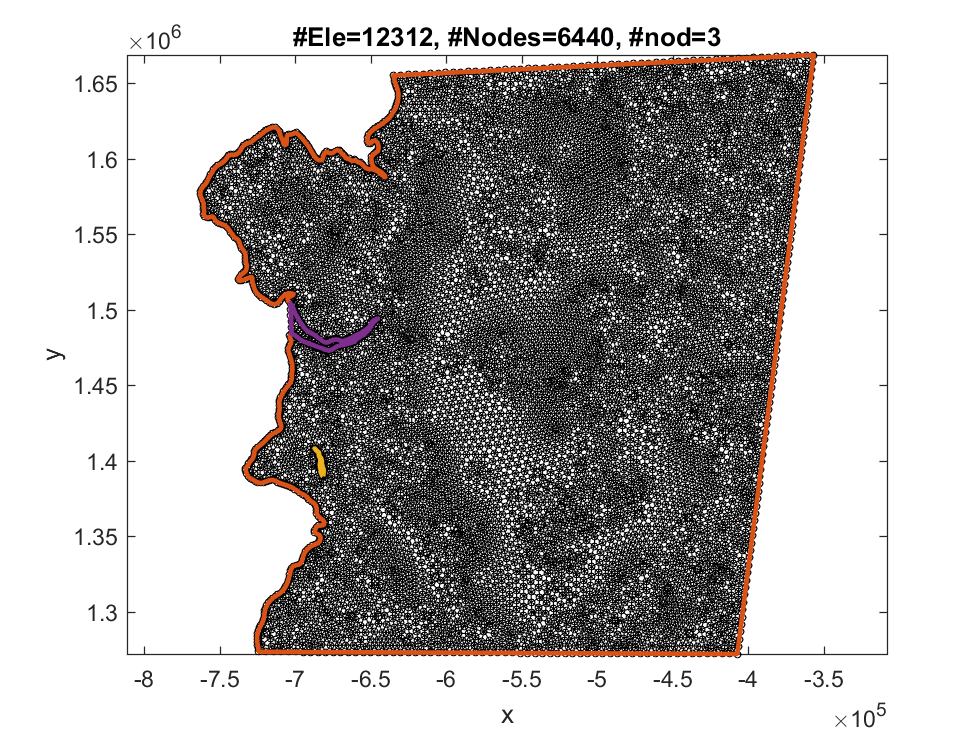
\includegraphics [width=4in]{ExamplesOfMeshGeneration_19.eps}



\end{document}
    
